\documentclass[11pt]{beamer} %Add 'handout' in the options for printing

\usepackage{beamercolorthemewolverine}
\usetheme{AnnArbor}

\usepackage[english]{babel}
\usepackage{amsmath,amssymb}
\usepackage{mathtools}
\usepackage{commath}
\usepackage{amssymb,amscd,amsfonts,amsbsy}
\usepackage{enumerate}
\usepackage{epsfig}
\usepackage{pgfpages}
\usepackage{graphics}
\usepackage{graphicx}
\usepackage{multicol}
\usepackage{layouts}
\usepackage[center]{caption}
\usepackage{natbib}
%\usepackage{movie15}
\usepackage{etex}
\usepackage[export]{adjustbox}
\usepackage{embedfile}
\usepackage{caption}
\usepackage{soul,xcolor}
\usepackage{import}
\usepackage{relsize}
\usepackage{tikz}
\usepackage[makeroom]{cancel}
\usepackage{multimedia}
\usepackage{subcaption}
\usepackage{comment}
%\usepackage{media9}



%Setup note page
\setbeamertemplate{note page}[plain]
%\setbeameroption{show notes on second screen=right}
%\setbeameroption{show notes on second screen=left}

\setbeamertemplate{navigation symbols}{}%remove navigation symbols

\setbeamertemplate{footline}[frame number]{}%gets rid of bottom navigation bars


\graphicspath{ {../figs/lung_figs/} }


% Figures within a column...
\makeatletter
\newenvironment{tablehere}
{\def\@captype{table}}
{}
\newenvironment{figurehere}
{\def\@captype{figure}}
{}
\makeatother

\newcommand{\beginbackup}{
   \newcounter{framenumbervorappendix}
   \setcounter{framenumbervorappendix}{\value{framenumber}}
}
\newcommand{\backupend}{
   \addtocounter{framenumbervorappendix}{-\value{framenumber}}
   \addtocounter{framenumber}{\value{framenumbervorappendix}} 
}

%---------------------------------------------------------------------------
%\setbeamercolor{mycolor}{fg=White,bg=White}
\setbeamercolor{alerted text}{fg=red} 
\setbeamertemplate{frametitle}
{
  \vskip-5pt 
  \leavevmode
  \begin{center}
    \vspace*{-0.5cm}
  \hbox{%
  \begin{beamercolorbox}[wd=0.85\paperwidth,ht=0.35cm,dp=1.35ex]{White}%
    \raggedright
    \vspace*{-.25cm}
    {\normalsize \insertframetitle} %\small{\insertframetitle}
  \end{beamercolorbox}
  % \hspace*{1em}{\normalsize \insertframetitle} %\small{\insertframetitle}
  }%
  \end{center}
  \vspace*{-0.75cm}
}
\def\newblock{\hskip .11em plus .33em minus .07em}

\setbeamertemplate{headline}{}

\setbeamercovered{dynamic}


\newcommand{\RR}{{\mathbb{R}}}
\newcommand{\NN}{{\mathbb{N}}}
\newcommand{\ZZ}{{\mathbb{Z}}}
\newcommand{\CC}{{\mathbb{C}}}
\newcommand{\eps}{\varepsilon}
\newcommand{\bp}{\noindent {\it Proof}.\,\,\,}
\newcommand{\ep}{\hfill$\Box$ \vskip 0.08in}
\newcommand{\dint}{\int\!\!\!\int}
\newcommand{\vs}{\vskip 0.5cm}
\newcommand{\po}{{\partial\Omega}}
\newcommand{\meanint}{{\int{\mkern-19mu}-}}
\def\ring{\mathaccent"0017 }

\definecolor{AliceBlue}{RGB}{240,248,255}


%\definecolor{lightblue}{rgb}{1,0,0}
%\sethlcolor{lightblue}
\renewcommand<>{\hl}[1]{\only#2{\beameroriginal{\hl}}{#1}}

% http://tex.stackexchange.com/questions/41683/why-is-it-that-coloring-in-soul-in-beamer-is-not-visible
\makeatletter
\newcommand\SoulColor{%
  \let\set@color\beamerorig@set@color
  \let\reset@color\beamerorig@reset@color}
\makeatother
\SoulColor



%\usepackage{media9}%
%\newcommand{\includemovies}[3]{%
%\includemedia[%
%width=#1,height=#2,%
%activate=pagevisible,%
%deactivate=pageclose,%
%addresource=#3,%
%flashvars={%
%src=#3 % same path as in addresource!
%&autoPlay=true % default: false; if =true, automatically starts playback after activation (see option ‘activation)’
%&loop=true % if loop=true, media is played in a loop
%&controlBarAutoHideTimeout=0 %  time span before auto-hide
%}%
%]{}{StrobeMediaPlayback.swf}%
%}



%%% Local Variables:
%%% mode: latex
%%% TeX-master: "../main"
%%% End:

\embedfile{\jobname}
\embedfile{include/preamble.tex}
% 

% My commands
\newcommand{\orderof}[1]{\ensuremath{\mathcal{O}\left(#1\right)}}
\newcommand{\plus}{\raisebox{.2\height}{\scalebox{.8}{+}}}
\newcommand{\minus}{\raisebox{.2\height}{\scalebox{.8}{-}}}
\newcommand{\timesx}{\raisebox{.2\height}{\scalebox{.8}{\times}}}
\newcommand{\equals}{\raisebox{.25\height}{\scalebox{0.9}{=}}}
\renewcommand{\CancelColor}{\color{red}} %change cancel color to red
\newcommand*\diff{\mathop{}\!\mathrm{d}}
\newcommand*\Diff[1]{\mathop{}\!\mathrm{d^#1}}
% \newcommand{\mycbox}[1]{\tikz{\path[draw=#1,fill=#1] (0,0) rectangle (1cm,1cm);}}


\makeatletter
% This is used for crossing out terms in an equation, but it works, but causes weird syntax errors when compiling that borks the terminal
\let\my@cancelto\cancelto %copy over the original cancelto command
\newcommand<>{\cancelto}[2]{\alt#3{\my@cancelto{#1}{#2}}{\mathrlap{#2}\phantom{\my@cancelto{#1}{#2}}}}
% redefine the cancelto command, using \phantom to assure that the
% result doesn't wiggle up and down with and without the arrow
\makeatother


\begin{document}
% %% Some customizations, based on https://tex.stackexchange.com/questions/22346/how-to-customize-titlepage-in-beamer

% \defbeamertemplate*{title page}{customized}[1][]
% {
% %  \usebeamerfont{title}\inserttitle\par
% %  \usebeamerfont{subtitle}\usebeamercolor[fg]{subtitle}\insertsubtitle\par
% %  \bigskip
%  % \usebeamerfont{author}\insertauthor\par
% %  \usebeamerfont{institute}\insertinstitute\par
% %  \usebeamerfont{date}\insertdate\par
%   \usebeamercolor[fg]{titlegraphic}\inserttitlegraphic
% }


%%
\title[]{Applications of Computation in Acoustics:\\Ultrasound Bioeffects \&\\ Underwater Transmission Loss Uncertainty}
\author[] {}

\institute[]{}
\date[date]{}


\begin{frame} %\vspace{1cm}
  \vspace*{1cm}
  %\titlepage \vspace{-2.50cm}

  {
    %\definecolor{darkpowderblue}{rgb}{0.0, 0.2, 0.6} %% UNCOMMENT IF NOT IN PREAMPLE
    \setbeamercolor{title}{fg=white, bg=darkpowderblue}
  \begin{beamercolorbox}[sep=8pt,center,wd=\paperwidth,ht=0.3\textheight,dp=0.045\textheight]{title}
    \usebeamerfont{title}\inserttitle\par%
  \end{beamercolorbox}
  }
  \centering
  \begin{columns}
    \column{.25\textwidth}
    
    % \begin{figure}\vspace*{1.3cm} \centering 
\includegraphics[width=.70\columnwidth]{include/figs/MichiganSeal} \end{figure}
    \column{.5\textwidth}
    \begin{center}
      % 
      \normalsize{A \emph{dissertation defense} by:\\Brandon Patterson} \vspace{16pt} \\ 
      % 
      \footnotesize{Scientific Computing and Flow Physics Lab} \vspace{4pt}\\
      \footnotesize{University of Michigan, Ann Arbor} \vspace{4pt}\\
      \scriptsize{Department of Mechanical Engineering} \vspace{4pt}\\
      % \scriptsize{$^2$Department of Radiology} \vspace{4pt}
    \end{center}
    \column{.25\textwidth}
    \vspace*{.15cm}
    % \begin{figure} \vspace*{1.3cm} \centering 
\includegraphics[width=.70\columnwidth]{include/figs/MElogo} \end{figure}
  \end{columns}
  \vspace{.25cm}
  \begin{center}
    % 
    % 
    %%%%%%%%%%%%%%%%%%% Put Date Here   %%%%%%%%%%%%%%%%%%%%%%%%%%%%
    % \footnotesize {\today} \vspace{-.1cm}
    \footnotesize {October 31, 2017} \vspace{-.1cm}
    % 
    % 
  \end{center}



  % 
  % 
  %%%%%%%%%%%%%%%%%%% FUNDING SOURCE OR CONFERENCE IMAGES BELOW ( L | C | R )   %%%%%%%%%%%%%%%%%%%%
  \begin{minipage}{\textwidth}
    \hspace*{.5cm}
    \begin{minipage}{.3\textwidth}
      \begin{center} 
        \begin{figure}
          \centering
          % \includegraphics[width=.4\textwidth]{include/figs/NIH_logo}
          %	\label{fig:NIH_logo_blue}
        \end{figure}
      \end{center}
    \end{minipage}
    \begin{minipage}{.3\textwidth}
      \begin{center} 
        \begin{figure}
          \centering
          % \includegraphics[width=.8\textwidth]{include/figs/nsfgrfp}
          \label{fig:NSF_logo_blue}
        \end{figure}
      \end{center}
    \end{minipage}
    \begin{minipage}{.3\textwidth}
      \begin{center} 
        
      \end{center}
    \end{minipage}
  \end{minipage}
\end{frame}
%%% Local Variables:
%%% mode: latex
%%% TeX-master: "../main"
%%% End:

\input{./slidedeck/asa_boston_2017_titleslide.tex }



%%%%%%%%%%%%%%%%%%%%%%%%%%%%%%%% Slides %%%%%%%%%%%%%%%%%%%%%%%%%%%%%%
\begin{frame}% \frametitle{\vspace*{0.5cm}Ultrasound-induced lung hemorrhage is not a new problem}
  \frametitle{\vspace*{0.5cm}Diagnostic ultrasound can trigger lung hemorrhage in mammals}
  {\small%
    \begin{itemize}%
    \item Lung Hemorrhage (LH) is the only known bioeffect of non-contrast DUS%
    \item Has been shown to occur in mice, rats, pigs, rabbits, monkeys \citep{Child1990,OBrien1997a,Tarantal1994a}.%
    \item The underlying physical damage mechanism is not understood.%
    \end{itemize}%
    % 
    \begin{figure}%
      \centering%
      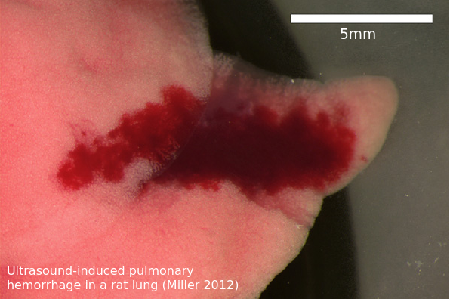
\includegraphics[width=0.5\textwidth]{LungBleed2} \nocite{Miller2012}%
    \end{figure}%
    %
%    The basic physical problem we have in the lungs is a mechanical wave interacting with an air-tissue interface.
    %\visible<2>{We aim to use computational modeling and simulations to investigate the underlying physics of DUS-induced LH.}%
    % 
  }
  \note{
    \begin{enumerate}
    \item DUS-induced LH isn't new.
    \item Has been shown to occur under clinically safe conditions in a variety of mammals
    \item Isn't a result of typical US bioeffect mechanisms
    \item Physical damage mechanism isn't understood.
    \end{enumerate}
  }
\end{frame}

%%% Local Variables:
%%% mode: latex
%%% TeX-master: "../main"
%%% End:

% 
\begin{frame}\frametitle{}
  {\Large Fundamental physical problem:\vspace*{0.25cm}\\ An acoustic wave
    interacting with a tissue-air interface}
  \captionsetup[subfigure]{labelformat=empty}
  \begin{figure}
    \centering
    \begin{tikzpicture}
      \tikzset{%
        box/.style    = { %rounded corners = 5pt,
          align           = left,
          font            = \sffamily\bfseries\large,
          text width      = 5.5cm, 
          blur shadow     = {shadow blur steps = 15} },    
        minimum height  = 0.4\textwidth
      }
      \node [box,
      fill         = pink, 
      text         = black,] 
      (T)
      {\quad Tissue \vspace{0.2\textwidth}\\%
        \includegraphics[width=\textwidth]{./figs/ultrasound_example_transparent}
      };
      \node [box, right  = 0cm of T, fill = blue!20!white] (A)
      {\quad Air \vspace*{0.65\textwidth}\\ \quad 
      };
    \end{tikzpicture}
  \end{figure}
  \pause
  We want to understand the dynamics of this problem
\end{frame}
% \begin{frame}
%   \begin{tikzpicture}
%     \tikz \fill[fill=black!20] 
%     plot[mark=triangle*,mark options={color=black,rotate=180}] 
%     file{plots/pgfmanual-sine.table} |- (0,0);
%   \end{tikzpicture}
% \end{frame}
% 
% 
\begin{frame}
  \vfill
  \textbf{Hypothesis:}\\Ultrasound waves generate baroclinic vorticity at gas-liquid interfaces, driving the interface deformation\\
  \vfill
  \pause
  \invisible<1>{
    Aims:
    \begin{enumerate}
    \item Test hypothesis \vspace{0.25cm} \pause%
    \item Simulate alveoli-like, gas-liquid interfaces driven by \textbf{clinically relevant} ultrasound waves \vspace{0.25cm} \pause%
    \item Calculate interface stresses and strains and compare with expected alveolar failure thresholds \vspace{0.25cm}%
    \end{enumerate}
  } \vfill
\end{frame}
% 
\input{./slidedeck/hypo_lung_new}
% 
\begin{frame} \frametitle{\mbox{\textit{Past work:} Acoustic waves are capable of deforming gas-liquid interfaces}}
  \begin{figure}
    \captionsetup[subfigure]{labelformat=empty}
    \centering
    \only<1>{
      \begin{subfigure}[b]{0.32\textwidth}
        \def\svgwidth{\textwidth}
        \import{../figs/avpaper_figs/}{trapezoidal_wave_asa_schematic.pdf_tex}%
        \vspace*{0.5cm}%
        \caption{Input pressure}
      \end{subfigure}
    }
    \only<2->{
      \begin{subfigure}[b]{0.33\textwidth}
        % \includegraphics[height=0.8\textwidth]{../figs/avpaper_figs/a0_t1000_24-May-2017}
        % \includegraphics[height=0.8\textwidth]{../figs/avpaper_figs/intf_amp_t1000_24-May-2017}
        \includegraphics[width=\textwidth]{../figs/avpaper_figs/intf_amp_t1000_asa_23-Jun-2017}
        \vspace*{0.5cm}%
        \caption{ $a(t) \sim t^{\nicefrac{3}{5}}$}
      \end{subfigure}
    }
    ~
    \begin{subfigure}[b]{0.3\textwidth}
      \begin{tikzpicture}
        \node[anchor=south west,inner sep=0] (image) at (0,0) {%
          \includegraphics[width=\textwidth]{./figs/snapshots_density_t1_t300_asa}
        };%
        \begin{scope}[x={(image.south east)},y={(image.north west)}]%
          \node[font=\scriptsize,align=left,right] at (0.1,0.92){{\textcolor{white}{Water}}};%
          \node[font=\scriptsize,align=left,right] at (0.1,0.5){{Air}};%
        \end{scope}%
      \end{tikzpicture}
      \caption{Density}
    \end{subfigure}
    ~
    % \hspace*{-0.85cm}
    \begin{subfigure}[b]{0.3\textwidth}
      % \hspace*{-0.85cm}
      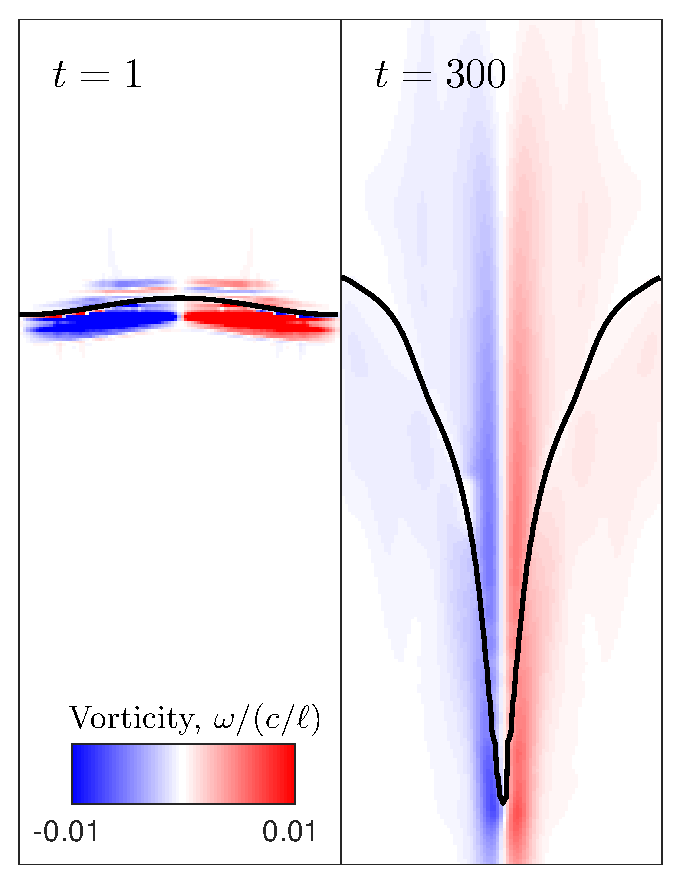
\includegraphics[width=0.84\textwidth]{./figs/vorticity_snapshots_asa_noax}%
      \vspace*{0.125cm}%
      \caption{Vorticity}
    \end{subfigure}
  \end{figure}
  \only<1>{
  A trapezoidal acoustic waves caused significant deformations of an
  almost flat air-water interfaces. Linear acoustics couldn't explain
  this.%
  }
  \only<2>{
  Interface deformation can be mathematically described in terms of vorticity, $\omega = \nabla \times \boldsymbol{u}$.
  }
  \vfill
  \scalebox{.5}{\scriptsize Patterson, B., \& Johnsen, E. (2016). Dynamics of an acoustically driven liquid-gas interface. J. Acoust. Soc. Am.}
\end{frame}
% 
\begin{frame}
  \frametitle{\vspace*{0.25cm}Ultrasound driven alveoli are modeled as compressible fluids.}
  \only<1-2>{
    \vspace*{0.5cm}
    \captionsetup[subfigure]{labelformat=empty,justification=centering}
    \begin{figure}
      \centering
      % \begin{subfigure}[b]{0.3\textwidth}
      %   \includegraphics[width=\textwidth]{./figs/lung_figs/alveolar_sac}
      %   %   \caption{A histological cross section of alveoli. [By Jpogi (Own work) [CC BY-SA 4.0
      %   (http://creativecommons.org/licenses/by-sa/4.0)], via Wikimedia
      %   Commons]}
      % \end{subfigure}
      \begin{subfigure}[b]{0.3\textwidth}
        \centering
        \includegraphics[width=\textwidth]{../figs/lung_figs/alveolar_sac}
        \vspace*{0.5cm}
        \def\svgwidth{\textwidth}
        {\small
          \import{../2016_acoustic_vorticity/figs/lung_figs/}{Alveolus_US_zoom_only_diagram.pdf_tex} \hfill%
        }
        \caption{\mbox{Physical problem schematic}}
      \end{subfigure}%
      %
      \visible<2>{%
        \begin{subfigure}[b]{0.69\textwidth}%
          \centering \def\svgwidth{\textwidth} {\footnotesize%
            \import{../2016_acoustic_vorticity/figs/lung_figs/}{usbe_model_schematic_domain_tall.pdf_tex}%
            \hfill%
          }%
          \caption{\label{fig:problem_schematic} Domain and model problem schematic.}%
        \end{subfigure}%
      }%
    \end{figure}
    {\tiny
      [By Jpogi (Own work) [CC BY-SA 4.0
      (http://creativecommons.org/licenses/by-sa/4.0)], via Wikimedia
      Commons]
    }
  }
  % 
  \only<3->{
    % \scriptsize{
    %   % \begin{align*}
    %   %   p(y,t_0) = p_a\sin{\left(2\pi f\frac{\left[y-\left(Y_{wave}+L_{wave}\right)\right]}{c}\right)}\exp{\left(-\frac{\left(\left[y-\left(Y_{wave}+L_{wave}/2\right)\right]c\right)^2}{FWHM/\left(2\sqrt{2\ln{\left(2\right)}} \right)}\right)}.%
    %   % \end{align*}
    % }
    \begin{figure}
      \centering
      \captionsetup[subfigure]{labelformat=empty}
      \begin{subfigure}[b]{0.4\textwidth}
        \includegraphics[width=\textwidth]{../figs/lung_figs/p0_vs_t_us}
        \vspace*{0.75cm}
        \caption{\label{fig:alveolar_histology} Ultrasound pulse
          waveform}
      \end{subfigure}
      \hfill
      \begin{subfigure}[b]{0.55\textwidth}
        \centering
        \def\svgwidth{\textwidth}%
        {\scriptsize \import{./figs/}{p_rho_ic_fields.pdf_tex}}%
        \caption{Initial Condition}
      \end{subfigure}
    \end{figure}
  }
  % 
  % \caption[A schematic view of the physical and model
  % problems]{\protect\subref{fig:alveolar_schematic} illustrates the
  % physical problem of interest, an ultrasound wave traveling into
  % the lung and impinging upon the first alveolus it
  % encounters. \subref{fig:problem_schematic} model problem,
  % consisting of an acoustic wave impinging from water onto a
  % sinusoidally interface with air. The left image shows the entire
  % domain and the right zooms in on the area around the interface.}
  % \label{fig:schematics}
\end{frame}
% 
% 
% 
% 
\begin{frame}
  \frametitle{\vspace*{0.25cm} The interface dynamics are simulated}
  \vspace*{0.5cm}
  Ex: Ultrasound pulse: $f=1.5$ MHz, $p_a=5$ MPa; Interface:$a_0=0.3\ell$.
  \begin{figure}
    \centering
    \begin{subfigure}[b]{0.9\textwidth}
      \begin{tikzpicture}
        \node[anchor=south west,inner sep=0] (image) at (0,0) {%
          \includegraphics[width=\textwidth]{../figs/lung_figs/rmawave_1_A50_a30_t500_rho_snapshots}
        };%
        \begin{scope}[x={(image.south east)},y={(image.north west)}]%
          \node[font=\scriptsize,align=left,right] at (0.06,0.92){{\textcolor{white}{Wave hits}}};%
          \node[font=\scriptsize,align=left,right] at (0.06,0.86){{\textcolor{white}{interface}}};%
          \node[font=\scriptsize,right] at (0.27,0.92){{\textcolor{white}{Wave leaves}}};%
          \node[font=\scriptsize,right] at (0.27,0.86){{\textcolor{white}{interface}}};%
        \end{scope}%
      \end{tikzpicture} 
    \end{subfigure}
  \end{figure}
  \begin{center}
    \begin{minipage}{0.75\linewidth}
      The interface evolves long after the wave has passed.\vspace*{0.25cm}\\%
      Linear acoustics can't explain this.
    \end{minipage}
  \end{center}
\end{frame}
% 
% 
\begin{frame}
  \vfill
  \textbf{Hypothesis:}\\Ultrasound waves generate baroclinic vorticity at gas-liquid interfaces, driving the interface deformation\\
  \vfill
  Aims:
  \begin{enumerate}
  \item Test hypothesis \vspace{0.25cm}%
  \end{enumerate}
  \vfill
  \pause
  {\Large Is the ultrasound-induced interface deformation driven by baroclinic vorticity?}
  \vfill
\end{frame}
% 
\begin{frame}
  \frametitle{\vspace*{0.5cm}Baroclinic vorticity is driving the deformation after the wave passes}
  Consider an air-water interface driven by a $10$ MPa ultrasound pulse
  \begin{figure}
    \centering
    \vfill
    \captionsetup[subfigure]{labelformat=empty}
    \begin{subfigure}[b]{0.3\textwidth}
      \centering
      \begin{tikzpicture}
        \node[anchor=south west,inner sep=0] (image) at (0,0) {%
          \includegraphics[height=\textwidth]{./figs/vorticity_t1_rmawave_1_5000000,0_0,1_45,0_0,0_1,0_1,0_50_100}
          \includegraphics[height=0.99\textwidth]{./figs/other_vorticity_plot}
        };%
        \begin{scope}[x={(image.south east)},y={(image.north west)}]%
          \node[font=\scriptsize,align=left,right] at (0.1,0.9){{$t=1$}};%
          \node[font=\scriptsize,align=left,right] at (0.55,0.9){{$t=20$}};%
        \end{scope}%
      \end{tikzpicture}
      \caption{Vorticity}
    \end{subfigure}
    \hfill
    \visible<2->{%
    \begin{subfigure}[b]{0.32\textwidth}
      \centering
      \begin{tikzpicture}
        \node[anchor=south west,inner sep=0] (image) at (0,0) {%
          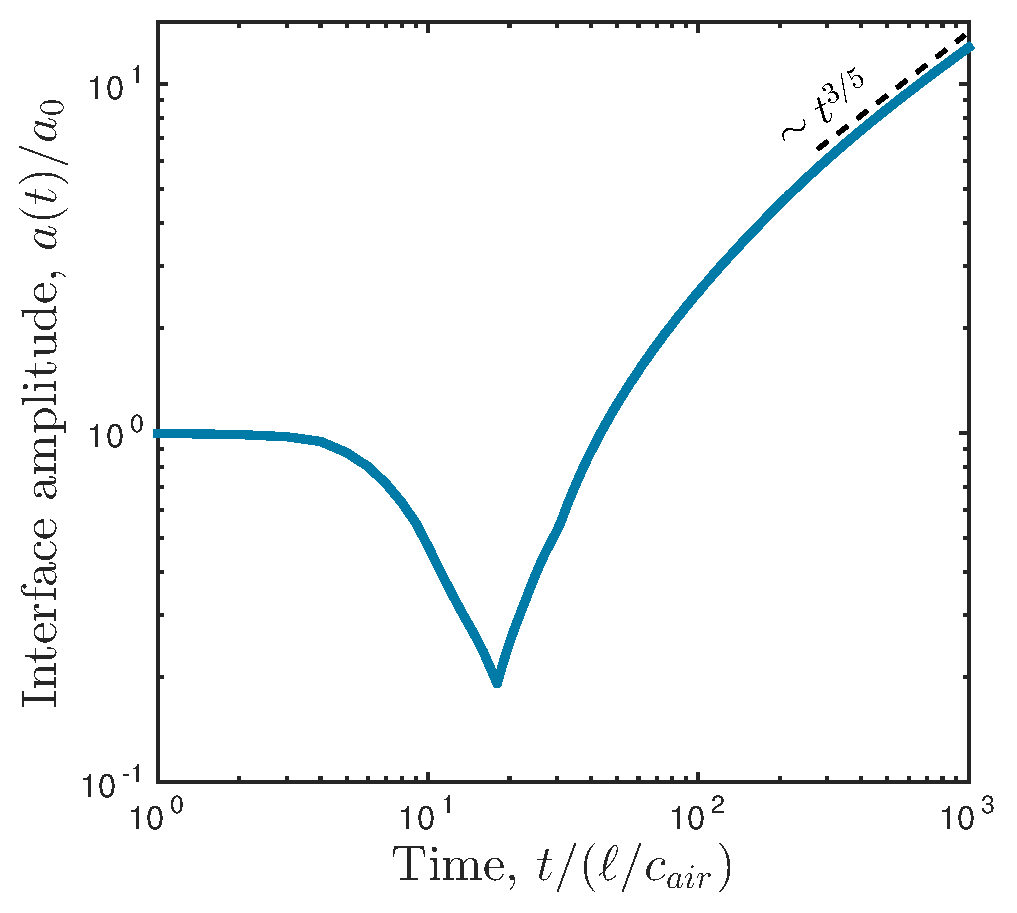
\includegraphics[width=\textwidth]{./figs/trapz_us_amp_comparison_A10_waveend_asa}
          %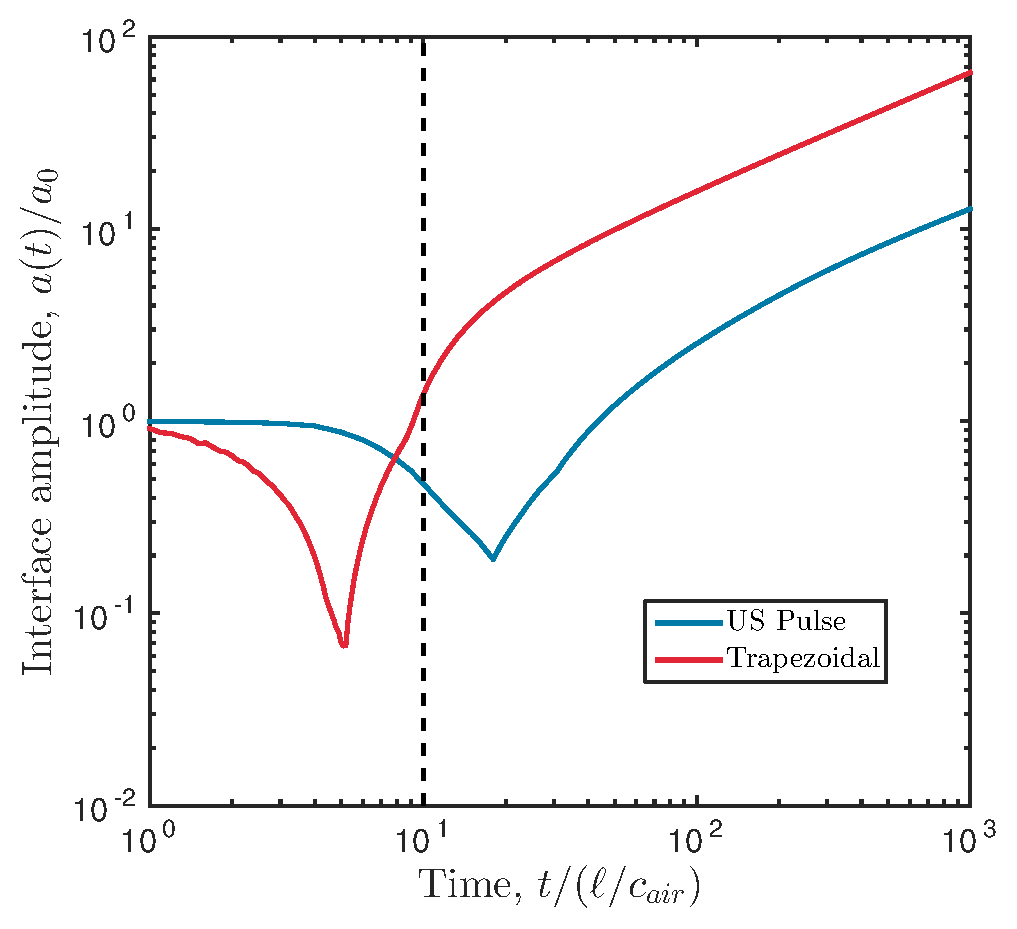
\includegraphics[width=\textwidth]{./figs/trapz_us_amp_comparison_A10_waveend}
        };%
        % \begin{scope}[x={(image.south east)},y={(image.north west)}]%
        %   \node[font=\scriptsize,align=left,right] at
        %   (0.2,0.9){{$t=1$}};%
        % \end{scope}%
      \end{tikzpicture}
      \caption{Interface growth $a(t)/a_0$}
    \end{subfigure}
    ~
    \begin{subfigure}[b]{0.32\textwidth}
      \begin{tikzpicture}
        \node[anchor=south west,inner sep=0] (image) at (0,0) {%
          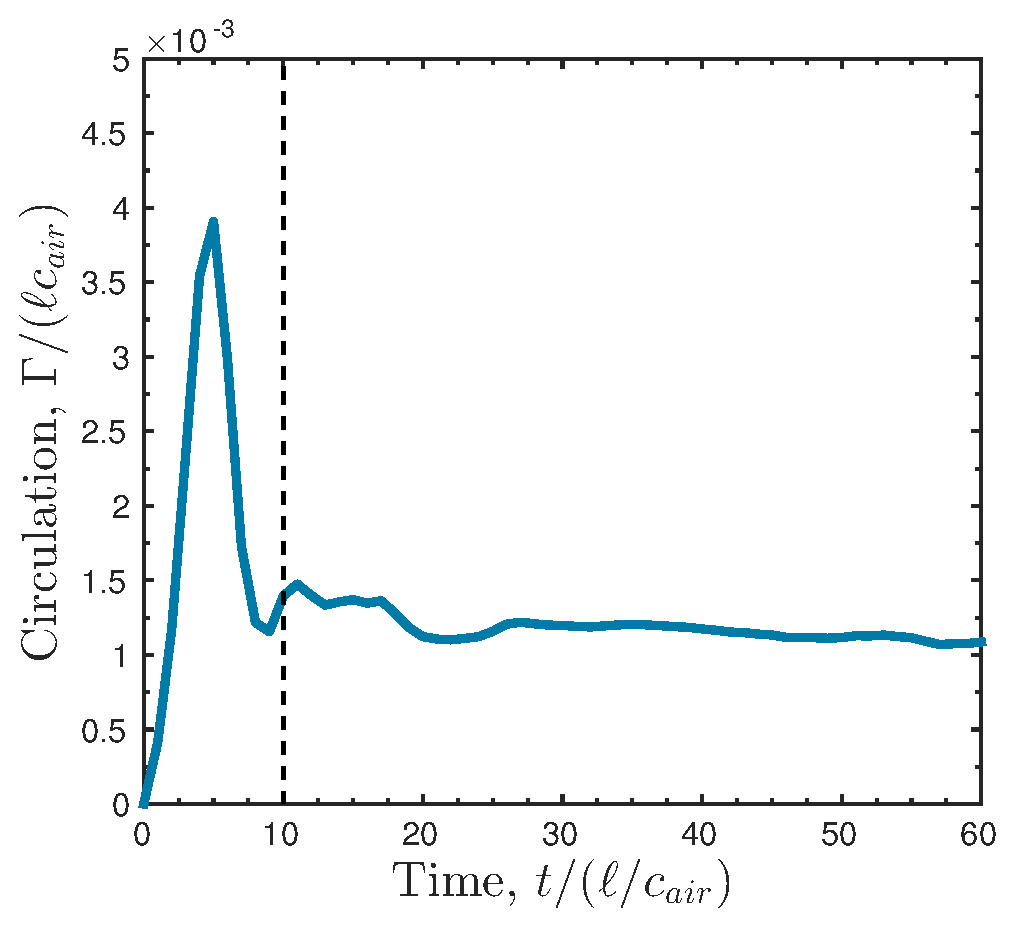
\includegraphics[width=\textwidth]{./figs/trapz_us_circ_comparison_A10_waveend_t0_t60_asa}
        };%
        % \begin{scope}[x={(image.south east)},y={(image.north west)}]%
        %   \node[font=\scriptsize,align=left,right] at
        %   (0.2,0.9){{$t=20$}};%
        % \end{scope}%
      \end{tikzpicture}
      \caption{Circulation, $\Gamma = \int_{A_R} \omega dA$}
    \end{subfigure}
    }
  \end{figure}
  Interface amplitude grows as $\approx t^{\nicefrac{3}{5}}$, at late times independently of the driving waveform\\
%  - Same order of magnitude circulation is deposited
\end{frame}
%
\begin{comment}
  \begin{frame}%
    \frametitle{The ultrasound pulse deposits baroclinic vorticity at
      the interface}%
    % \includegraphics[width=0.8\textwidth]{./figs/vorticity_t1_t10_rmawave_1_5000000.0_0.1_45.0_0.0_1.0_1.0_50_100}
    \vspace*{1cm}
    \begin{figure}
      \centering \vfill
      \captionsetup[subfigure]{labelformat=empty}
      \begin{subfigure}[b]{0.3\textwidth}
        \centering
        \begin{tikzpicture}
          \node[anchor=south west,inner sep=0] (image) at (0,0) {%
            \includegraphics[width=\textwidth]{./figs/vorticity_t1_rmawave_1_5000000,0_0,1_45,0_0,0_1,0_1,0_50_100}
          };%
          \begin{scope}[x={(image.south east)},y={(image.north
              west)}]%
            \node[font=\scriptsize,align=left,right] at
            (0.2,0.9){{$t=1$}};%
          \end{scope}%
        \end{tikzpicture}
        \caption{During the wave}
      \end{subfigure}
      \hspace*{1cm}
      \begin{subfigure}[b]{0.3\textwidth}
        \begin{tikzpicture}
          \node[anchor=south west,inner sep=0] (image) at (0,0) {%
            \includegraphics[width=0.91\textwidth]{./figs/other_vorticity_plot}
          };%
          \begin{scope}[x={(image.south east)},y={(image.north
              west)}]%
            \node[font=\scriptsize,align=left,right] at
            (0.2,0.9){{$t=20$}};%
          \end{scope}%
        \end{tikzpicture}
        \caption{After the wave}
      \end{subfigure}
    \end{figure}
  \end{frame}
% 
% 
  \begin{frame}
    \frametitle{\vspace*{0.5cm}Baroclinic vorticity deforms
      ultrasound-driven interfaces}
    Comparing the $10$ MPa ultrasound pulse and trapezoidal waves:
    \begin{figure}
      \centering \vfill
      \captionsetup[subfigure]{labelformat=empty}
      \begin{subfigure}[b]{0.48\textwidth}
        \centering
        \begin{tikzpicture}
          \node[anchor=south west,inner sep=0] (image) at (0,0) {%
            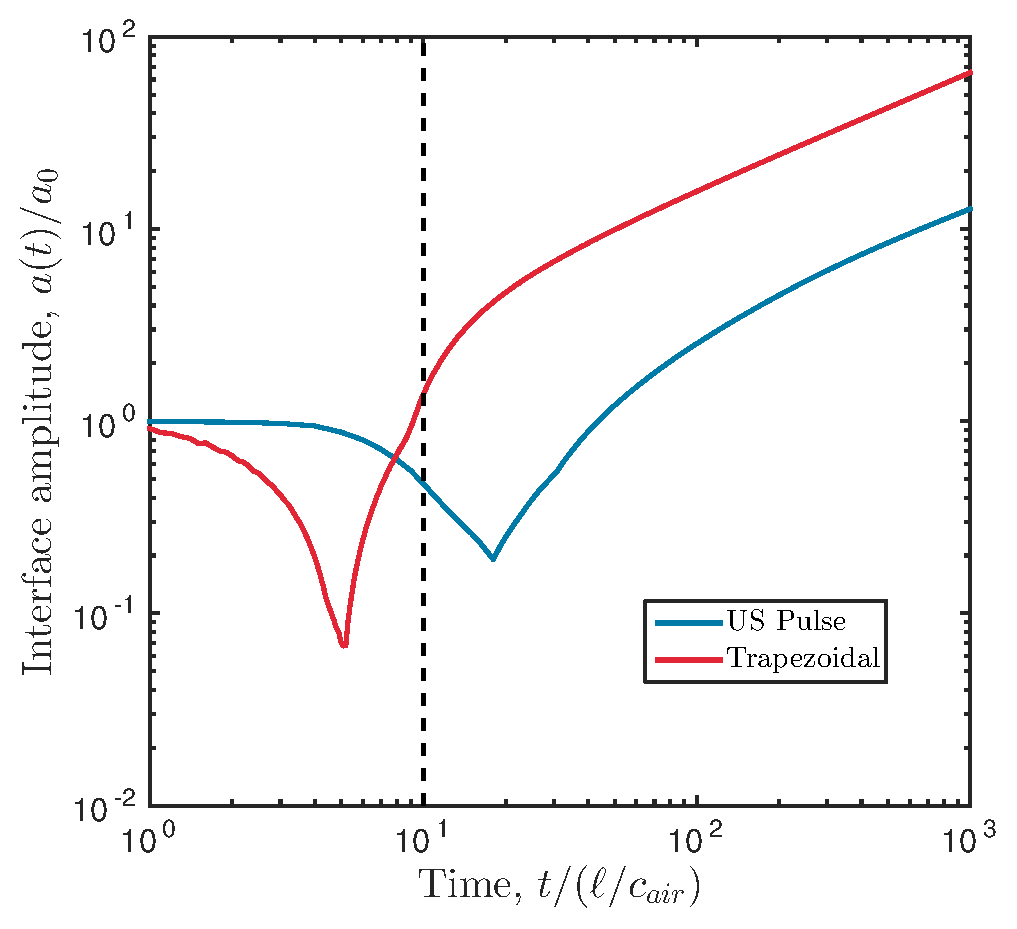
\includegraphics[width=\textwidth]{./figs/trapz_us_amp_comparison_A10_waveend}
          };%
          % \begin{scope}[x={(image.south east)},y={(image.north
          %   west)}]%
          %   \node[font=\scriptsize,align=left,right] at
          %   (0.2,0.9){{$t=1$}};%
          % \end{scope}%
        \end{tikzpicture}
        \caption{Interface growth $a(t)/a_0$}
      \end{subfigure}
      ~
      \begin{subfigure}[b]{0.48\textwidth}
        \begin{tikzpicture}
          \node[anchor=south west,inner sep=0] (image) at (0,0) {%
            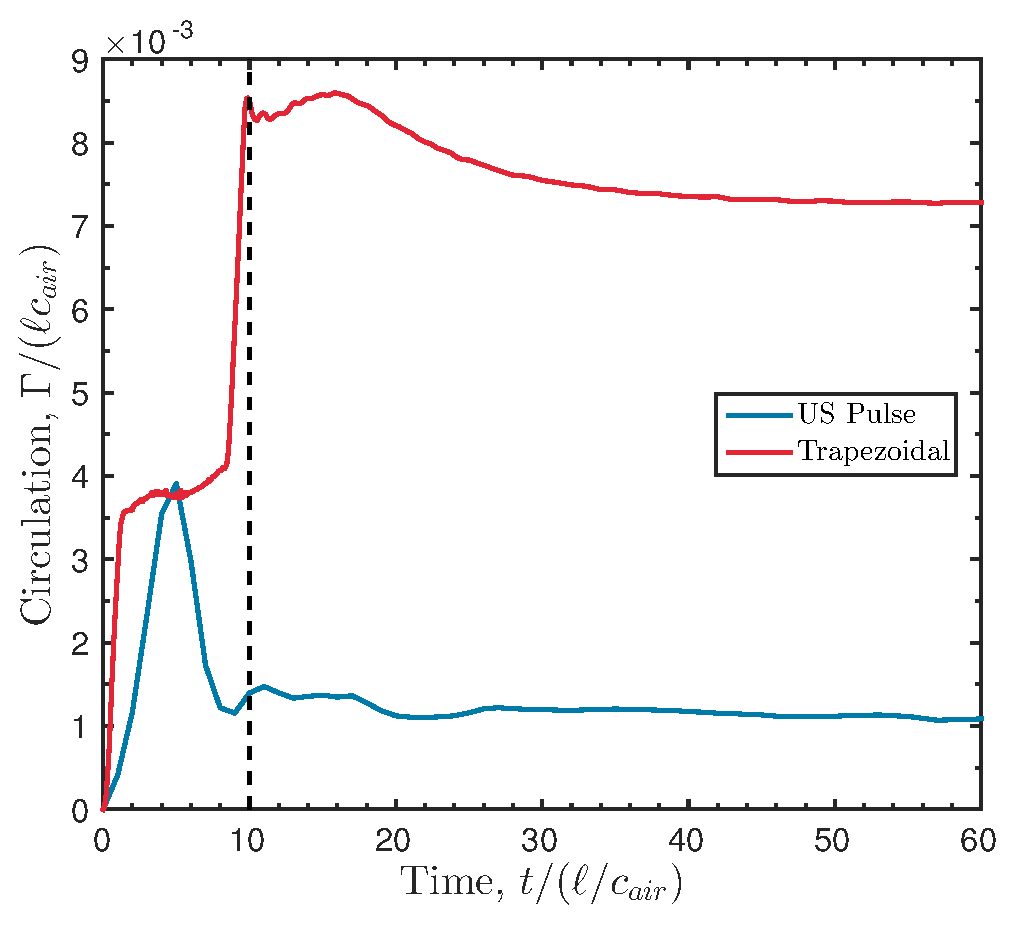
\includegraphics[width=\textwidth]{./figs/trapz_us_circ_comparison_A10_waveend_t0_t60}
          };%
          % \begin{scope}[x={(image.south east)},y={(image.north
          %   west)}]%
          %   \node[font=\scriptsize,align=left,right] at
          %   (0.2,0.9){{$t=20$}};%
          % \end{scope}%
        \end{tikzpicture}
        \caption{Circulation, $\Gamma = \int_{A_R} \omega dA$}
      \end{subfigure}
    \end{figure}
    - Interface amplitude grows as $\approx t^{\nicefrac{3}{5}}$ independent of waveform\\
    - Same order of magnitude circulation is deposited
  \end{frame}
\end{comment}

% 
% 
\begin{frame}
  % So far, this hasn't been very relevant to clinical ultrasound
\end{frame}
% 
% 
\begin{frame}\frametitle{\vspace*{0.5cm}Now let's consider the more clinically relevant cases}
  \hspace*{0.22cm}Wave and interface perturbation amplitudes are varied.%
  \begin{figure}
    \captionsetup[subfigure]{labelformat=empty}
    \centering
    \begin{subfigure}[b]{0.5\textwidth}
      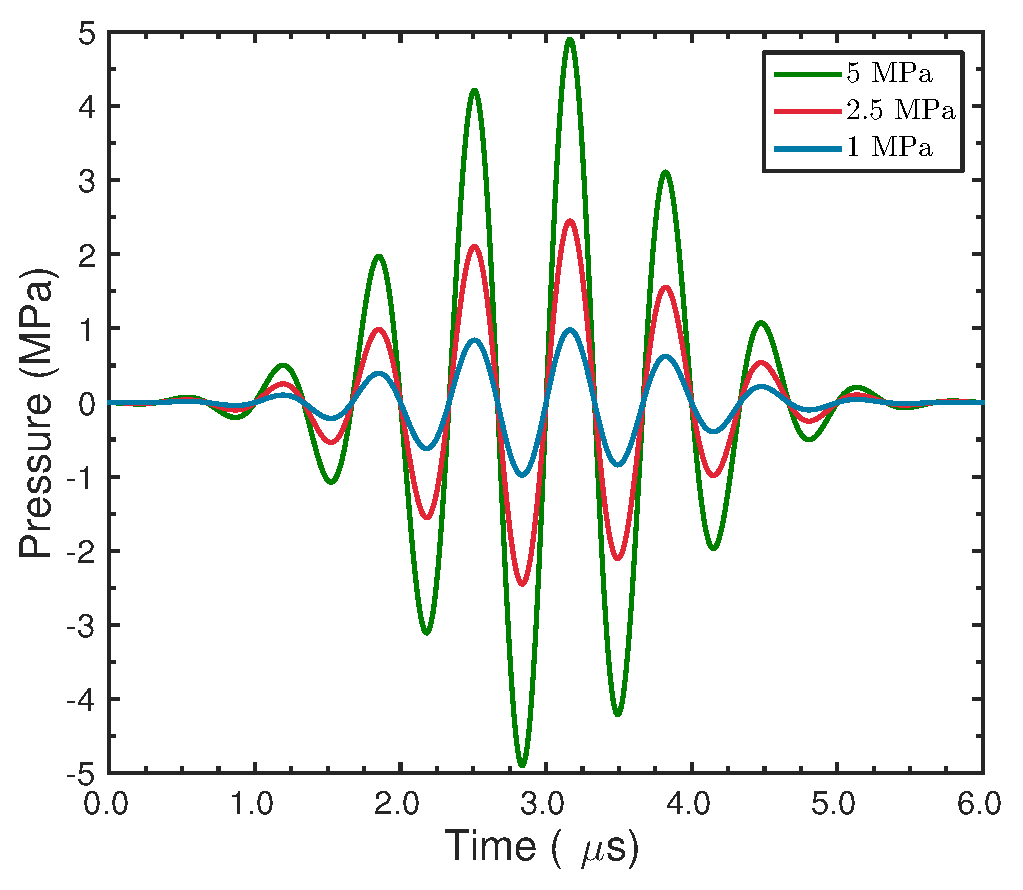
\includegraphics[width=0.9\textwidth]{./figs/us_pulse_amps_dim}
      \caption{Ultrasound Pulses}
    \end{subfigure}
    \hspace*{0.5cm}
    \visible<2>{%
    \begin{subfigure}[b]{0.35\textwidth}%
      \begin{tikzpicture}%
        \node[anchor=south west,inner sep=0] (image) at (0,0) {%
          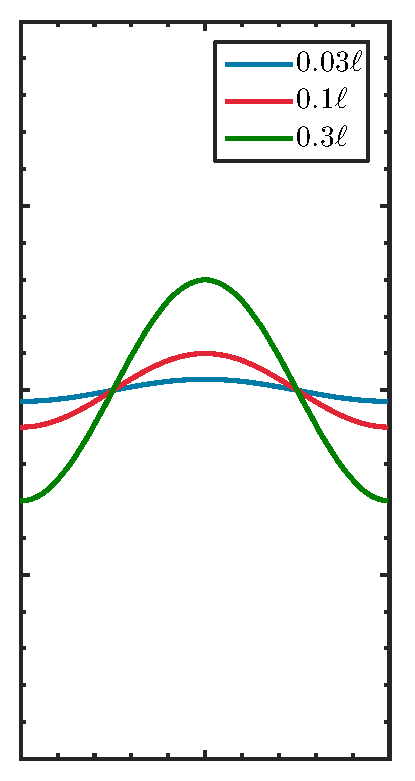
\includegraphics[width=0.5\textwidth]{./figs/us_intf_amps_dim}%
        };%
        \begin{scope}[x={(image.south east)},y={(image.north west)}]%
          \node[font=\small,align=right,left] at (0.0,1){{$\ell$}};%
          \node[font=\small,align=right,left] at (0.0,0.75){{$\ell/2$}};%
          \node[font=\small,align=right,left] at (0.0,0.5){{$0$}};%
          \node[font=\small,align=right,left] at (0.0,0.25){{$-\ell/2$}};%
          \node[font=\small,align=right,left] at (0.0,0){{$-\ell$}};%
          \node[font=\small,align=right,left] at (0.15,-0.02){{$0$}};%
          \node[font=\small,align=right,left] at (1.1,-0.04){{$\ell$}};%
        \end{scope}%
      \end{tikzpicture}%
      \caption{\quad Interface initial conditions}%
    \end{subfigure}%
    }%
  \end{figure}%
  \vspace*{-0.25cm}%
  \begin{itemize}%
  \item Assume typical alveolar diameter $\ell = 200 \mu$m \citep{Ochs2004} \vspace*{4pt}%
  \item Pulse amplitudes, $p_a = 1, 2.5, 5$ MPa;\,\, frequency, $f = 1.5$ MHz  \vspace*{4pt}%
    \visible<2>{%
  \item Interface perturbation amplitudes $a_0 = 0.03\ell, 0.10\ell, 0.30\ell$  \vspace*{4pt}%
  }%
  \end{itemize}
\end{frame}
% 
% 
\begin{frame}\frametitle{\vspace*{0.5cm}The inferred viscous stress is calculated}
  \begin{center}
    $\tau_{xy}(x,y,t) = \mu\left(\frac{\partial u}{\partial y}+ \frac{\partial v}{\partial x}\right)$,
    \qquad$p_a = 5$ MPa
  \end{center}
  \begin{figure}
    \captionsetup[subfigure]{labelformat=empty}
    \centering
    \begin{subfigure}[b]{0.3\textwidth}
      \begin{tikzpicture}%
        \node[anchor=south west,inner sep=0] (image) at (0,0) {
          \includegraphics[width=\textwidth]{../figs/lung_figs/rmawave_1_A50_a03_t005_tauxy_snapshots_dim}
        };%
        \begin{scope}[x={(image.south east)},y={(image.north west)}]%
          \node[font=\small,right] at (0.2,0.9) {$\tau_{xy}$ (Pa)};%
          \node[font=\small,right] at (0.2,0.25) {$t = 2.9 \mu$s };%
        \end{scope}%  
      \end{tikzpicture}%
      \caption{\label{fig:tauxy_snapshot_A50_a03} $a_0 = 0.03\ell$}
    \end{subfigure}
    ~ 
    \begin{subfigure}[b]{0.3\textwidth}
      \begin{tikzpicture}%
        \node[anchor=south west,inner sep=0] (image) at (0,0) {
          \includegraphics[width=\textwidth]{../figs/lung_figs/rmawave_1_A50_a10_t005_tauxy_snapshots_dim}
        };%
        \begin{scope}[x={(image.south east)},y={(image.north west)}]%
          \node[font=\small,right] at (0.2,0.9) {$\tau_{xy}$ (Pa)};%
          \node[font=\small,right] at (0.2,0.25) {$t = 2.9 \mu$s };%
        \end{scope}%  
      \end{tikzpicture}%
      \caption{\label{fig:tauxy_snapshot_A50_a10} $a_0 = 0.1\ell$}
    \end{subfigure}
    ~ 
    \begin{subfigure}[b]{0.3\textwidth}
      \begin{tikzpicture}%
        \node[anchor=south west,inner sep=0] (image) at (0,0) {
          \includegraphics[width=\textwidth]{../figs/lung_figs/rmawave_1_A50_a30_t500_tauxy_snapshots_dim}
        };%
        \begin{scope}[x={(image.south east)},y={(image.north west)}]%
          \node[font=\small,right] at (0.2,0.9) {$\tau_{xy}$ (Pa)};%
          \node[font=\small,right] at (0.2,0.25) {$t = 2.9 \mu$s };%
        \end{scope}%  
      \end{tikzpicture}%
      \caption{\label{fig:tauxy_snapshot_A50_a30} $a_0 = 0.3\ell$}
    \end{subfigure}
    % 
  \end{figure}
  \begin{itemize}
  \item Viscous shear stresses are concentrated at the interface
  \item The maximum shear stress, occurs approximately when the peak negative pressure hits the interface
  \end{itemize}
\end{frame}
% 
% 
\begin{frame}\frametitle{\vspace*{0.5cm}The inferred viscous stress is calculated}
  \begin{center}
    $\tau_{xy}(x,y,t) = \mu\left(\frac{\partial u}{\partial y}+ \frac{\partial v}{\partial x}\right)$,
    \qquad$a_0 = 0.3\ell$ MPa
  \end{center}
  \begin{figure}
    \captionsetup[subfigure]{labelformat=empty}
    \begin{subfigure}{0.5\textwidth}
      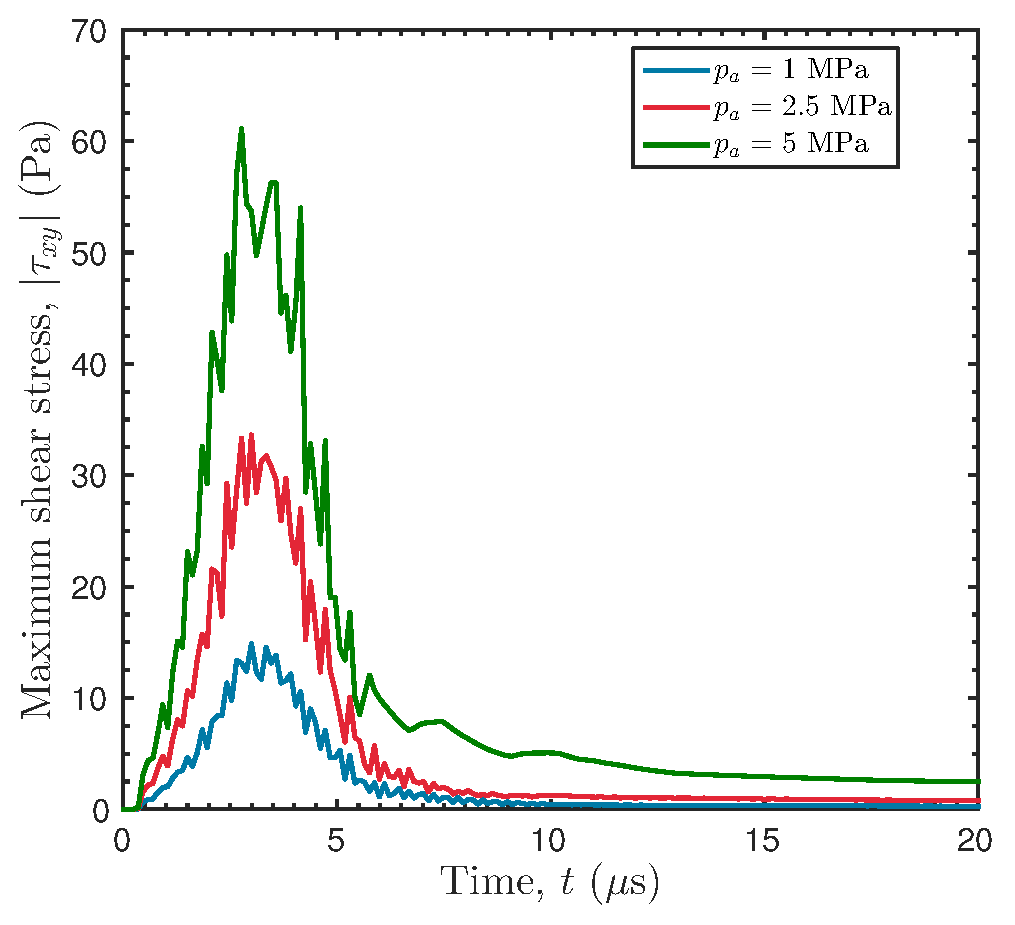
\includegraphics[width=\textwidth]{../figs/lung_figs/rmawave_1_A10,25,50_a30_tauxy_dim_15-Jun-2017}
    \end{subfigure}
    % \caption{$a_0 = 0.3\ell$ MPa}
  \end{figure}
  \vspace*{-0.25cm}
  \begin{itemize}
  \item Maximum calculated shear stress, $\approx 50$ Pa 
  \item $\approx$ alveolar wall stress failure criterion, $8$ kPa \citep{West1991}
  \end{itemize}
\end{frame}
% 
% 
\begin{frame}\frametitle{\vspace*{0.5cm}The interface strain is calculated}
  \begin{center}
    $\varepsilon(t) = \frac{s(t)-s_0}{s_0},    \qquad s = \text{arclength of interface}$
  \end{center}
  \begin{figure}
    \captionsetup[subfigure]{labelformat=empty}
    \centering
    % \begin{subfigure}[b]{0.49\textwidth}
    %   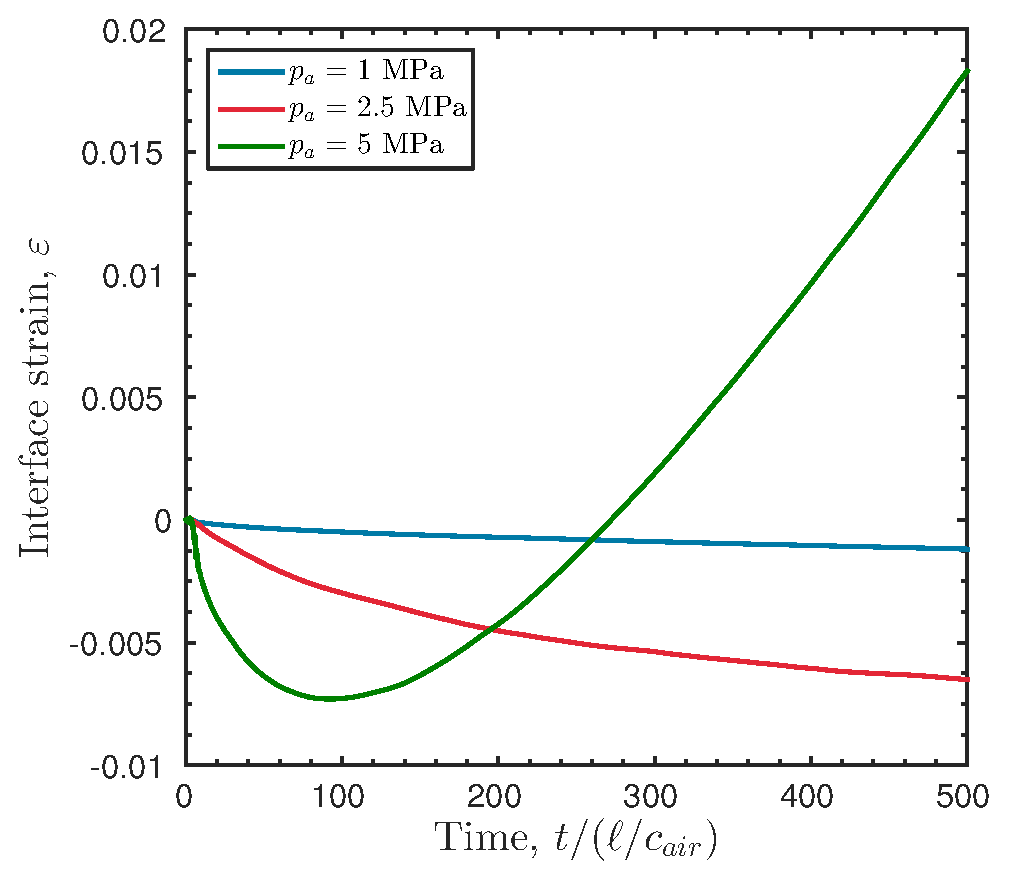
\includegraphics[width=\textwidth]{../figs/lung_figs/rmawave_1_A10,25,50_a03_strain_08-Mar-2017}
    %   \caption{\label{fig:strain_multi-pa_a03} $a_0 = 0.03\ell$}
    % \end{subfigure}
    % ~ 
    \begin{subfigure}[b]{0.45\textwidth}
      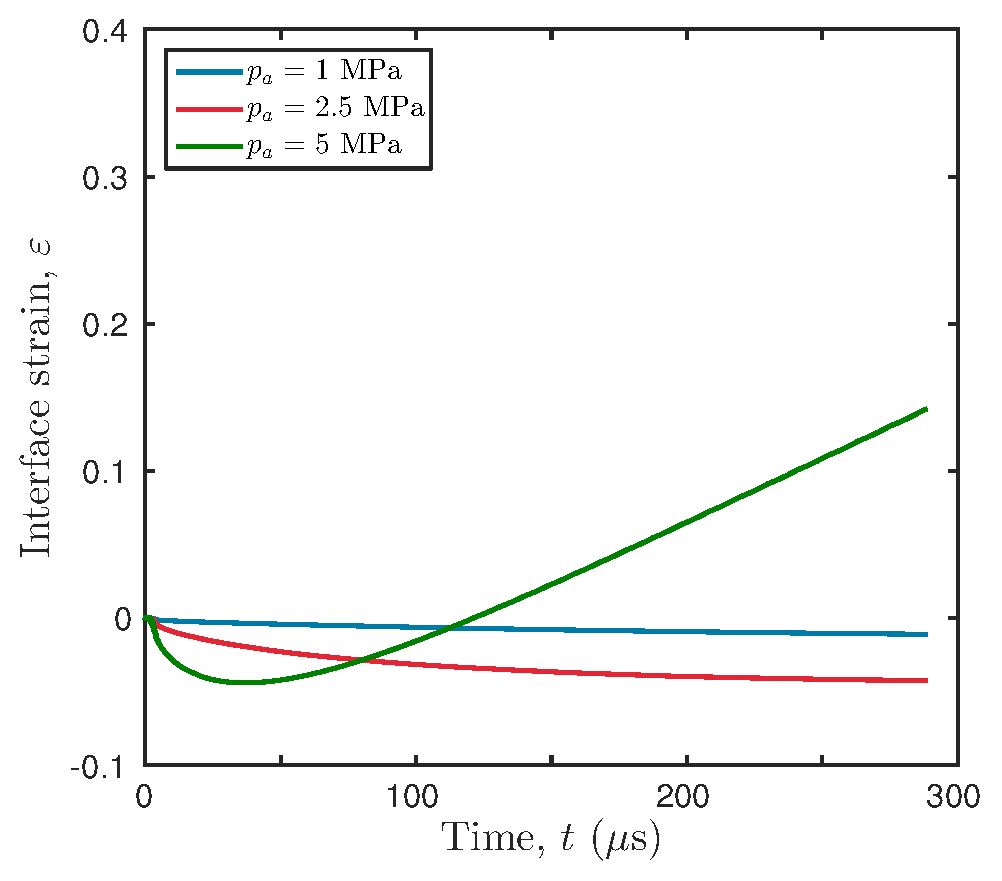
\includegraphics[width=\textwidth]{../figs/lung_figs/rmawave_1_A10,25,50_a10_strain_15-Jun-2017_dim}
      \caption{\label{fig:strain_multi-pa_a30} $a_0 = 0.1\ell$}
    \end{subfigure}
    ~
    \begin{subfigure}[b]{0.45\textwidth}
      \includegraphics[width=\textwidth]{../figs/lung_figs/rmawave_1_A10,25,50_a30_strain_15-Jun-2017_dim}
      \caption{\label{fig:strain_multi-pa_a30} $a_0 = 0.3\ell$}
    \end{subfigure}
  \end{figure}
  \vspace*{-0.25cm}
  \begin{itemize}
  \item Strain increases with increasing $p_a$ and $a_0$
  \item For $a_0=0.3\ell$ and $p_a = 1, 2.5,$ and $5$ MPa maximum strains, at $t \approx 300\mu$s, are $\varepsilon =-0.01, -0.05,$ and $0.38$ respectively.
  \item $\approx$ alveolar strain failure criterion, $\varepsilon = ?$.
  \end{itemize}
\end{frame}
% 
% 
\begin{frame}\frametitle{Discussion and conclusions}%
  \vfill
  \begin{itemize}
  \item A single ultrasound pulse is sufficient to appreciably strain
    an air-water interface via baroclinic vorticity.\vfill
  \item Newtonian viscous stress alone is not likely to cause
    hemorrhage.\vfill  
  \item Circulation from subsequent pulses could add up.\vfill
  \item Better characterization of mechanical properties (e.g, elasticity, viscosity) is needed.\vfill
  \end{itemize}
  \vfill
\end{frame}
% 
% 
% \begin{frame}\frametitle{Conclusions}%
%   \vfill
%   \begin{itemize}
%   \item I need to finish these slides
%   \end{itemize}
%   \vfill
% \end{frame}
% 
% 
%%%%%%%%%%%%%%%%%%%%%%%%%%%%%%%%%%%%%%%%%%%%%%%%%%%%%%%%%%%%%%%%%%%%%%%%%%%%%% 
%%%%%%%%%%%%%%%%%%%%%%%%%%%%%%%%%%%%%%%%%%%%%%%%%%%%%%%%%%%%%%%%%%%%%%%%%%%%%% 
%%%%%%%%%%%%%%%%%%%%%%%%%%%%%%%%%%%%%%%%%%%%%%%%%%%%%%%%%%%%%%%%%%%%%%%%%%%%%% 
%%%%%%%%%%%%%%%%%%%%%%%%%%%%%%%%%%%%%%%%%%%%%%%%%%%%%%%%%%%%%%%%%%%%%%%%%%%%%% 
%%%%%%%%%%%%%%%%%%%%%%%%%%%%%%%%%%%%%%%%%%%%%%%%%%%%%%%%%%%%%%%%%%%%%%%%%%%%%% 
%%%%%%%%%%%%%%%%%%%%%%%%%%%%%%%%%%%%%%%%%%%%%%%%%%%%%%%%%%%%%%%%%%%%%%%%%%%%%% 
%%%%%%%%%%%%%%%%%%%%%%%%%%%%%%%%%%%%%%%%%%%%%%%%%%%%%%%%%%%%%%%%%%%%%%%%%%%%%% 
%%%%%%%%%%%%%%%%%%%%%%%%%%%%%%%%%%%%%%%%%%%%%%%%%%%%%%%%%%%%%%%%%%%%%%%%%%%%%% 
%%%%%%%%%%%%%%%%%%%%%%%%%%%%%%%%%%%%%%%%%%%%%%%%%%%%%%%%%%%%%%%%%%%%%%%%%%%%%% 
%%%%%%%%%%%%%%%%%%%%%%%%%%%%%%%%%%%%%%%%%%%%%%%%%%%%%%%%%%%%%%%%%%%%%%%%%%%%%% 
%%%%%%%%%%%%%%%%%%%%%%%%%%%%%%%%%%%%%%%%%%%%%%%%%%%%%%%%%%%%%%%%%%%%%%%%%%%%%% 
%%%%%%%%%%%%%%%%%%%%%%%%%%%%%%%%%%%%%%%%%%%%%%%%%%%%%%%%%%%%%%%%%%%%%%%%%%%%%% 
%%%%%%%%%%%%%%%%%%%%%%%%%%%%%%%%%%%%%%%%%%%%%%%%%%%%%%%%%%%%%%%%%%%%%%%%%%%%%% 
%%%%%%%%%%%%%%%%%%%%%%%%%%%%%%%%%%%%%%%%%%%%%%%%%%%%%%%%%%%%%%%%%%%%%%%%%%%%%% 
%%%%%%%%%%%%%%%%%%%%%%%%%%%%%%%%%%%%%%%%%%%%%%%%%%%%%%%%%%%%%%%%%%%%%%%%%%%%%% 
%%%%%%%%%%%%%%%%%%%%%%%%%%%%%%%%%%%%%%%%%%%%%%%%%%%%%%%%%%%%%%%%%%%%%%%%%%%%%% 
%%%%%%%%%%%%%%%%%%%%%%%%%%%%%%%%%%%%%%%%%%%%%%%%%%%%%%%%%%%%%%%%%%%%%%%%%%%%%% 
%%%%%%%%%%%%%%%%%%%%%%%%%%%%%%%%%%%%%%%%%%%%%%%%%%%%%%%%%%%%%%%%%%%%%%%%%%%%%% 
%%%%%%%%%%%%%%%%%%%%%%%%%%%%%%%%%%%%%%%%%%%%%%%%%%%%%%%%%%%%%%%%%%%%%%%%%%%%%% 
%%%%%%%%%%%%%%%%%%%%%%%%%%%%%%%%%%%%%%%%%%%%%%%%%%%%%%%%%%%%%%%%%%%%%%%%%%%%%% 
%%%%%%%%%%%%%%%%%%%%%%%%%%%%%%%%%%%%%%%%%%%%%%%%%%%%%%%%%%%%%%%%%%%%%%%%%%%%%% 
%%%%%%%%%%%%%%%%%%%%%%%%%%%%%%%%%%%%%%%%%%%%%%%%%%%%%%%%%%%%%%%%%%%%%%%%%%%%%% 
%%%%%%%%%%%%%%%%%%%%%%%%%%%%%%%%%%%%%%%%%%%%%%%%%%%%%%%%%%%%%%%%%%%%%%%%%%%%%% 
%%%%%%%%%%%%%%%%%%%%%%%%%%%%%%%%%%%%%%%%%%%%%%%%%%%%%%%%%%%%%%%%%%%%%%%%%%%%%% 
%%%%%%%%%%%%%%%%%%%%%%%%%%%%%%%%%%%%%%%%%%%%%%%%%%%%%%%%%%%%%%%%%%%%%%%%%%%%%% 
%%%%%%%%%%%%%%%%%%%%%%%%%%%%%%%%%%%%%%%%%%%%%%%%%%%%%%%%%%%%%%%%%%%%%%%%%%%%%% 
%%%%%%%%%%%%%%%%%%%%%%%%%%%%%%%%%%%%%%%%%%%%%%%%%%%%%%%%%%%%%%%%%%%%%%%%%%%%%% 
%%%%%%%%%%%%%%%%%%%%%%%%%%%%%%%%%%%%%%%%%%%%%%%%%%%%%%%%%%%%%%%%%%%%%%%%%%%%%% 
%%%%%%%%%%%%%%%%%%%%%%%%%%%%%%%%%%%%%%%%%%%%%%%%%%%%%%%%%%%%%%%%%%%%%%%%%%%%%% 
%%%%%%%%%%%%%%%%%%%%%%%%%%%%%%%%%%%%%%%%%%%%%%%%%%%%%%%%%%%%%%%%%%%%%%%%%%%%%% 
%%%%%%%%%%%%%%%%%%%%%%%%%%%%%%%%%%%%%%%%%%%%%%%%%%%%%%%%%%%%%%%%%%%%%%%%%%%%%% 
%%%%%%%%%%%%%%%%%%%%%%%%%%%%%%%%%%%%%%%%%%%%%%%%%%%%%%%%%%%%%%%%%%%%%%%%%%%%%% 
%%%%%%%%%%%%%%%%%%%%%%%%%%%%%%%%%%%%%%%%%%%%%%%%%%%%%%%%%%%%%%%%%%%%%%%%%%%%%% 
%%%%%%%%%%%%%%%%%%%%%%%%%%%%%%%%%%%%%%%%%%%%%%%%%%%%%%%%%%%%%%%%%%%%%%%%%%%%%% 
%%%%%%%%%%%%%%%%%%%%%%%%%%%%%%%%%%%%%%%%%%%%%%%%%%%%%%%%%%%%%%%%%%%%%%%%%%%%%% 
%%%%%%%%%%%%%%%%%%%%%%%%%%%%%%%%%%%%%%%%%%%%%%%%%%%%%%%%%%%%%%%%%%%%%%%%%%%%%% 
%%%%%%%%%%%%%%%%%%%%%%%%%%%%%%%%%%%%%%%%%%%%%%%%%%%%%%%%%%%%%%%%%%%%%%%%%%%%%% 
%%%%%%%%%%%%%%%%%%%%%%%%%%%%%%%%%%%%%%%%%%%%%%%%%%%%%%%%%%%%%%%%%%%%%%%%%%%%%% 
%%%%%%%%%%%%%%%%%%%%%%%%%%%%%%%%%%%%%%%%%%%%%%%%%%%%%%%%%%%%%%%%%%%%%%%%%%%%%% 
%%%%%%%%%%%%%%%%%%%%%%%%%%%%%%%%%%%%%%%%%%%%%%%%%%%%%%%%%%%%%%%%%%%%%%%%%%%%%% 
%%%%%%%%%%%%%%%%%%%%%%%%%%%%%%%%%%%%%%%%%%%%%%%%%%%%%%%%%%%%%%%%%%%%%%%%%%%%%% 
%%%%%%%%%%%%%%%%%%%%%%%%%%%%%%%%%%%%%%%%%%%%%%%%%%%%%%%%%%%%%%%%%%%%%%%%%%%%%% 



\begin{comment}
  % 
  \begin{frame} \frametitle{\vspace*{0.25cm} Shock-driven fluid-fluid interfaces have been studied extensively}
  {\small
    \hfill%
    \begin{figure}
      \centering
      \begin{tikzpicture}%
        \node[anchor=south west,inner sep=0] (image) at (0,0) {
          \def\svgwidth{0.6\textwidth}%
          \import{../figs/lung_figs/}{brouillette_fig3_mod_compact.pdf_tex}\hfill%
        };%
        \begin{scope}[x={(image.south east)},y={(image.north west)}]%
          \node[font=\tiny,right] at (0.15,-0.05) {\textcolor{black}{Adapted from \cite{Brouillette2002}}};%
        \end{scope}%  
      \end{tikzpicture}%
      \hfill
      \centering
      \begin{tikzpicture}%
        \node[anchor=south west,inner sep=0] (image) at (0,0) {
          \includegraphics[height=0.5\textheight]{../figs/lung_figs/baroclinic_schematic_vertical}%
        };%
        \begin{scope}[x={(image.south east)},y={(image.north west)}]%
          \node[font=\tiny,right] at (0.05,-0.05) {\textcolor{black}{Adapted from \cite{Heifetz2015}}};%
        \end{scope}%  
      \end{tikzpicture}%
    \end{figure}
    \hfill
    \begin{itemize}
    \item Shocks deposit baroclinic vorticity at perturbed fluid-fluid interfaces \citep{Drake2006}.
    \item This vorticity drives the interface perturbation to grow.
    \item This is the Richtymyer-Meshkov ``instability''.
    \item Acoustic waves are different. They interact over a finite time-scale.
    %\item This problem is not well studied for acoustic waves.
    \end{itemize}
  }
  \note{
      {\footnotesize
      \begin{enumerate}
      \item Shock interaction with perturbed fluid-fluid interfaces has been studied.
      \item This is RM
      \item Misalignments between pressure and density gradients cause a
        local rotation in the fluid. This is called baroclinic
        vorticity.
      \item Demo with basketball: Think of this basketball as fluid
        particle, and pretend its heavier on one side than the other.
        If wind hits it, the heavier side will accelerate slower than
        the light side and the basketball will rotate.
      \item This happens at across interfaces where the density changes.
      \item This rotation in the fluid accelerates different parts of
        the perturbation in different directions, and the
        perturbation grows.
      \item Shocks take place over few molecular mfps and pass quickly.
      \item This is a mechanism that provides a way for pressure waves
        such as shocks or acoustic waves to deform a fluid-fluid
        interface.
      \item Acoustic waves are fundamentally different in that they
        their interaction with a point on the interface takes up a
        finite amount of time.
      \item And this problem isn't studies well for acoustic waves.
      \end{enumerate}
      }
    }
  \end{frame}

%%% Local Variables:
%%% mode: latex
%%% TeX-master: "../main"
%%% End:


  \begin{frame}
    \frametitle{\vspace*{0.5cm}The model is adapted for acoustically-driven gas-liquid interfaces}
    \begin{figure}
      \centering
      \centering%
      \begin{subfigure}[b]{0.53\textwidth}
        \centering
        \def\svgwidth{\textwidth}%
        \import{../figs/avpaper_figs/}{shock_2_ultrasound_logic.pdf_tex}%
        \vspace*{2cm}
        \caption{Design of the trapezoidal waveform}
      \end{subfigure}
      \begin{subfigure}[b]{0.46\textwidth}
        \centering
        \def\svgwidth{\textwidth}
        {\footnotesize
          \import{../figs/avpaper_figs/}{p0_vs_y.pdf_tex}%
        }
        \caption{Acoustic pressure waveform}
      \end{subfigure}
    \end{figure}
    A trapezoidal wave is used to capture features of both the ultrasound pulse and the shock wave.
  \end{frame}


  % 
  % 
  \begin{frame} \frametitle{\vspace*{0.25cm}Problem setup remains otherwise unchanged}
    \vspace*{0.5cm}
    \begin{figure}
      \centering \def\svgwidth{0.6\textwidth} {\footnotesize
        \import{../2016_acoustic_vorticity/figs/lung_figs/}{usbe_model_schematic_domain_tall.pdf_tex}
      }
      \caption{\label{fig:problem_schematic} Domain and model problem
        schematic.}
    \end{figure}
  \end{frame}
  % 
  % 
  \begin{frame}
    \frametitle{The theoretical interface dynamics are calculated for trapezoidal waves of varying amplitude $p_a=5, 7.5, 10,$ and $12.5$ MPa.} 
    \begin{figure}
      \centering
      \begin{subfigure}[b]{0.6\textwidth}
        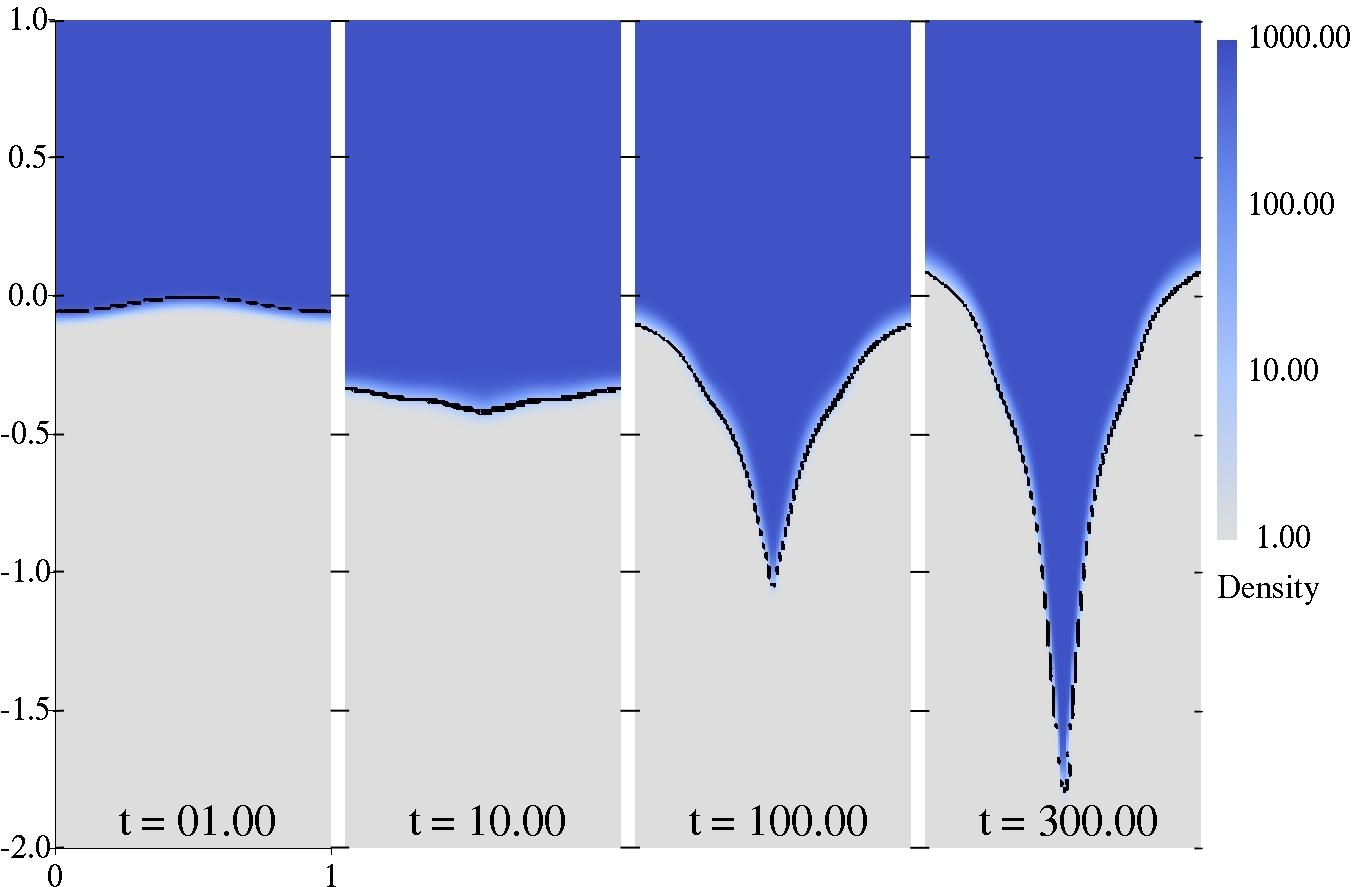
\includegraphics[width=\textwidth]{../2016_acoustic_vorticity/figs/lung_figs/snapshots_density_t1}
        \caption{$p_a = 10$ MPa.}
      \end{subfigure}
      \only<1>{
        \begin{subfigure}[b]{0.35\textwidth}
          \centering
          \includegraphics[width=\textwidth]{../2016_acoustic_vorticity/figs/lung_figs/trapz10_intf_schematic}%
          \caption{$0\leq t \leq 25$.}
        \end{subfigure}
      }
      \only<2>{
        \begin{subfigure}[b]{0.35\textwidth}
          \centering
          \includegraphics[width=\textwidth]{../2016_acoustic_vorticity/figs/lung_figs/trapz10_intf_t1000}%
          \caption{$0\leq t \leq 1000$.}
        \end{subfigure}
      }
    \end{figure}

  \end{frame}
  % 
  % 
  \begin{frame}%
    \frametitle{It is shown that baroclinic vorticity is capable of deforming the interface long after the wave has passed.}%
    \begin{figure}
      \centering
      \begin{subfigure}[b]{0.6\textwidth}
        \includegraphics[width=0.98\textwidth]{../2016_acoustic_vorticity/figs/lung_figs/vorticity_snapshot_mat}
        \caption{$p_a = 10$ MPa.}
      \end{subfigure}
      \only<1>{
        \begin{subfigure}[b]{0.35\textwidth}
          \centering
          $\Gamma = \int_{A_r} \omega dA_r$
          \includegraphics[height=0.9\textwidth]{../2016_acoustic_vorticity/figs/lung_figs/trapz10_circ_schematic.pdf}%
          \caption{$0\leq t \leq 25$.}
          \hfill
        \end{subfigure}
      }
      \only<2>{
        \begin{subfigure}[b]{0.35\textwidth}
          \centering
          $\Gamma = \int_{A_r} \omega dA_r$
          \includegraphics[height=0.9\textwidth]{../2016_acoustic_vorticity/figs/lung_figs/Gamma_t1000_28-Oct-2016}%
          \caption{$0\leq t \leq 1000$.}
          \hfill
        \end{subfigure}
      }
    \end{figure}
  \end{frame}
  % 
  % 
  \begin{frame}
    \frametitle{The interface perturbation appears to grow asymptotically.}
    \begin{minipage}{0.45\textwidth}
      \begin{figure}
        \centering
        \begin{subfigure}[t]{\textwidth}
          \centering
          \includegraphics[height=0.8\textwidth]{../2016_acoustic_vorticity/figs/lung_figs/a0_t1000_23-Dec-2016}
          \caption*{\label{fig:trapz_interface_t1000} Constant scaling:
            $a(t)/a_0$}
        \end{subfigure}
      \end{figure}
    \end{minipage}
    ~
    \begin{minipage}{0.45\textwidth}
      \only<2->{
        From dimensional analysis:
        \begin{align*}
          a(t) &\sim f\left(\Gamma, s,\ell,c\right)\\
          \text{We suspect}\\
          a(t) &\sim f\left(\frac{\Gamma}{s},\ell,c\right),\\
          \text{such that}\\
          \frac{a(t)}{\ell} &\sim \left(\frac{\Gamma}{s c}\right)\left(\frac{c}{\ell}t\right)^n
        \end{align*}
      }
    \end{minipage}



  \end{frame}
  % 
  % 
  \begin{frame}
    \frametitle{The interface perturbation amplitude grows approximately as $t^{3/5}$ and scales with the linear circulation density $\Gamma_0/s_0$.}
    \begin{figure}
      \centering
      \begin{subfigure}[t]{0.45\textwidth}
        \centering
        \includegraphics[height=0.8\textwidth]{../2016_acoustic_vorticity/figs/lung_figs/a0_t1000_23-Dec-2016}
        \caption{\label{fig:trapz_interface_t1000} Constant scaling: $a(t)/a_0$}
      \end{subfigure}
      ~
      \begin{subfigure}[t]{0.45\textwidth}
        \centering
        \includegraphics[height=0.8\textwidth]{../2016_acoustic_vorticity/figs/lung_figs/intf_amp_t1000_23-Dec-2016}
        \caption{Vortex strength scaling: $a(t)/\left(\frac{\Gamma_0}{s_0}\frac{\ell}{c}\right)$}
      \end{subfigure}
    \end{figure}
    The perturbation amplitude curves collapse by:\\
    (1) Syncing the time of the phase inversion\\ 
    (2) Scaling by $\Gamma / s$ at the time when circulation dominates the wave.
  \end{frame}
  % 
  % 
  \begin{frame}
    \frametitle{The interface arc length per unit circulation $s(t)/\Gamma(t)$ grows approximately as $t^{1/2}$ and scales with wave amplitude $p_a$.}
    \begin{figure}
      \centering
      \begin{subfigure}[t]{0.45\textwidth}
        \centering
        \includegraphics[height=0.8\textwidth]{../2016_acoustic_vorticity/figs/lung_figs/s_t1000_14-Feb-2017}
        \caption{\label{fig:trapz_interface_t1000} Constant scaling: $s(t)/\ell$}
      \end{subfigure}
      ~
      \begin{subfigure}[t]{0.45\textwidth}
        \centering
        \includegraphics[height=0.8\textwidth]{../2016_acoustic_vorticity/figs/lung_figs/scp_t1000_23-Dec-2016}
        \caption{Vortex strength scaling: $\frac{s(t)}{\Gamma(t)}\frac{p_a}{\rho c}$}
      \end{subfigure}
    \end{figure}
  \end{frame}
  % 
  % 
  % \begin{frame}
  %   \frametitle{The circulation deposited and therefore late time perturbation growth depend heavily on time-dependent wave features}
  %   \begin{figure}
  %     \centering
  %     \begin{subfigure}{0.49\textwidth}
  %       \includegraphics[width=\textwidth]{../2016_acoustic_vorticity/figs/lung_figs/interface_multi-lag}
  %       \caption{$a(t)/a_0$}
  %     \end{subfigure}
  %     \begin{subfigure}{0.49\textwidth}
  %       \includegraphics[width=\textwidth]{../2016_acoustic_vorticity/figs/lung_figs/circulation_multi-lag_fixed}
  %       \caption{$\Gamma(t)$}
  %     \end{subfigure}
  %     \begin{flushleft}
  %       {\footnotesize
  %       The interface amplitude (left) and circulation (right) histories
  %       for waves of varying total length $L$ and elevated static pressure
  %       duration between the expansion and compression. Here we show
  %       results for $L=45\ell$ (blue), $L=35\ell$ (orange), $L=30\ell$
  %       (yellow), $L=20\ell$ (purple), $L=15\ell$ (green), $L=10\ell$
  %       (light blue)
  %     }
  %     \end{flushleft}
  %     \label{fig:trapz_circ_interface_multi-lag}
  %   \end{figure}
  % \end{frame}
  % 
  \begin{frame} \frametitle{\vspace*{0.5cm}Summary and conclusions}
  \small
  Summary:
  \begin{itemize}
  \item We studied the interaction of finite-duration acoustic waves with gas-liquid interfaces.
  \end{itemize}
  \vspace*{0.25cm}
  Conclusions
  \begin{itemize}
  \item Baroclinic vorticity is generated acoustic wave-interface interactions%
  \item This vorticity appears to deforming perturbed liquid-gas interfaces.%
  \item The interface perturbation grows as $t^{3/5}$ and scales with linear circulation density along the interface $\Gamma_0 / s_0$.
  \item The interface arc length per unit circulation $s(t)/\Gamma(t)$ grows approximately as $t^{1/2}$ and scales with wave amplitude $p_a$.
  \item This may be a mechanism for ultrasound-induced alveolar strain and hemorrhage and should be studied further.
  \end{itemize}
\end{frame}
%%% Local Variables:
%%% mode: latex
%%% TeX-master: "../main"
%%% End:

  % 

  \begin{frame} \frametitle{\mbox{\textit{Past work:} Acoustic waves are capable of deforming gas-liquid interfaces \citep{Patterson2016}}}
    \begin{figure}
      \centering
      \begin{subfigure}[b]{0.48\textwidth}
        \def\svgwidth{\textwidth}
        \import{../figs/avpaper_figs/}{trapezoidal_wave_asa_schematic.pdf_tex}%
      \end{subfigure}
      \hfill
      \begin{subfigure}[b]{0.48\textwidth}
        \begin{tikzpicture}
          \node[anchor=south west,inner sep=0] (image) at (0,0) {%
            \includegraphics[width=0.8\textwidth]{../figs/lung_figs/snapshots_density_t1_t300}
          };%
          \begin{scope}[x={(image.south east)},y={(image.north west)}]%
            \node[font=\scriptsize,align=left,right] at (0.1,0.92){{\textcolor{white}{Water}}};%
            \node[font=\scriptsize,align=left,right] at (0.1,0.5){{Air}};%
          \end{scope}%
        \end{tikzpicture}
      \end{subfigure}
    \end{figure}
    A trapezoidal acoustic waves caused significant deformations of an
    almost flat air-water interfaces. Linear acoustics couldn't explain
    this.
  \end{frame}
  \begin{frame} \frametitle{\mbox{\textit{Past work:} Acoustic waves are capable of deforming gas-liquid interfaces}}
    \begin{figure}
      \centering
      \captionsetup[subfigure]{labelformat=empty}
      \begin{subfigure}[b]{0.45\textwidth}
        \includegraphics[width=\textwidth]{./figs/vorticity_snapshots_asa}
      \end{subfigure}
      % \begin{subfigure}[b]{0.45\textwidth}
      %   \includegraphics[width=\textwidth]{../figs/avpaper_figs/s_t1000_24-May-2017}
      %   \caption{\label{fig:trapz_scp_t1000_unscaled} Interface arc length: $s(t) \sim \Gamma(t) t^{\nicefrac{1}{2}}$}
      % \end{subfigure}
      \begin{subfigure}[b]{0.45\textwidth}
        % \includegraphics[height=0.8\textwidth]{../figs/avpaper_figs/a0_t1000_24-May-2017}
        \includegraphics[height=0.8\textwidth]{../figs/avpaper_figs/intf_amp_t1000_24-May-2017}
        \caption{ $a(t) \sim t^{\nicefrac{3}{5}}$}
      \end{subfigure}
    \end{figure}
    Vorticity drives deformation in a mathematically describable wave.
  \end{frame}
\end{comment}

%%%%%%%%%%%%%%%%%%%%%%%%%%%%%%%%%%%%%%%%%%%%%% 
% \begin{frame}  
%   \centering
%   \begin{center}
%     {\LARGE EXTRA SLIDES}\\
%   \end{center}
% \end{frame}
% \input{./slidedeck/pastwork_bubble}
% \begin{frame}
  \centering
  \begin{center}
    {\LARGE Part II: Current Project}\\
    
    Diagnostic ultrasound-induced lung hemorrhage and acoustic wave
    interactions with liquid-gas interfaces
  \end{center}
\end{frame}

%%% Local Variables:
%%% mode: latex
%%% TeX-master: "../main"
%%% End:

% \begin{frame} \frametitle{\vspace*{0.25cm} Shock-driven fluid-fluid interfaces have been studied extensively}
  {\small
    \hfill%
    \begin{figure}
      \centering
      \begin{tikzpicture}%
        \node[anchor=south west,inner sep=0] (image) at (0,0) {
          \def\svgwidth{0.6\textwidth}%
          \import{../figs/lung_figs/}{brouillette_fig3_mod_compact.pdf_tex}\hfill%
        };%
        \begin{scope}[x={(image.south east)},y={(image.north west)}]%
          \node[font=\tiny,right] at (0.15,-0.05) {\textcolor{black}{Adapted from \cite{Brouillette2002}}};%
        \end{scope}%  
      \end{tikzpicture}%
      \hfill
      \centering
      \begin{tikzpicture}%
        \node[anchor=south west,inner sep=0] (image) at (0,0) {
          \includegraphics[height=0.5\textheight]{../figs/lung_figs/baroclinic_schematic_vertical}%
        };%
        \begin{scope}[x={(image.south east)},y={(image.north west)}]%
          \node[font=\tiny,right] at (0.05,-0.05) {\textcolor{black}{Adapted from \cite{Heifetz2015}}};%
        \end{scope}%  
      \end{tikzpicture}%
    \end{figure}
    \hfill
    \begin{itemize}
    \item Shocks deposit baroclinic vorticity at perturbed fluid-fluid interfaces \citep{Drake2006}.
    \item This vorticity drives the interface perturbation to grow.
    \item This is the Richtymyer-Meshkov ``instability''.
    \item Acoustic waves are different. They interact over a finite time-scale.
    %\item This problem is not well studied for acoustic waves.
    \end{itemize}
  }
  \note{
      {\footnotesize
      \begin{enumerate}
      \item Shock interaction with perturbed fluid-fluid interfaces has been studied.
      \item This is RM
      \item Misalignments between pressure and density gradients cause a
        local rotation in the fluid. This is called baroclinic
        vorticity.
      \item Demo with basketball: Think of this basketball as fluid
        particle, and pretend its heavier on one side than the other.
        If wind hits it, the heavier side will accelerate slower than
        the light side and the basketball will rotate.
      \item This happens at across interfaces where the density changes.
      \item This rotation in the fluid accelerates different parts of
        the perturbation in different directions, and the
        perturbation grows.
      \item Shocks take place over few molecular mfps and pass quickly.
      \item This is a mechanism that provides a way for pressure waves
        such as shocks or acoustic waves to deform a fluid-fluid
        interface.
      \item Acoustic waves are fundamentally different in that they
        their interaction with a point on the interface takes up a
        finite amount of time.
      \item And this problem isn't studies well for acoustic waves.
      \end{enumerate}
      }
    }
  \end{frame}

%%% Local Variables:
%%% mode: latex
%%% TeX-master: "../main"
%%% End:

% \begin{frame}
  
\end{frame}
%%% Local Variables:
%%% mode: latex
%%% TeX-master: "../main"
%%% End:

% \begin{frame}
  \Large
  We aim to use fluid mechanics with computational modeling and simulations to investigate the underlying physics of DUS-lung interaction:\\
  \vspace*{0.5cm}
  Acoustic wave interactions with liquid-gas interfaces.
\end{frame}
%%% Local Variables:
%%% mode: latex
%%% TeX-master: "../main"
%%% End:

% \begin{frame} \frametitle{We hypothesize that US waves generate baroclinic vorticity at air-tissue interfaces in the lungs, straining fragile alveolar walls.}%
  \visible<2->{
    The vorticity generation equation\vspace{2pt}
    \only<2>{
      \scalebox{1.0}{$
        \frac{\partial \boldsymbol{\omega}}{\partial t}%
        +\left(\boldsymbol{u}\cdot\nabla\right)\boldsymbol{\omega}=% 
        \left(\boldsymbol{\omega}\cdot\nabla\right)\boldsymbol{u}%
        -\boldsymbol{\omega}\left(\nabla\cdot\boldsymbol{u}\right)%
        +\frac{\nabla\rho\times\nabla p}{\rho^2}%
        -\nabla\times\left(\frac{\nabla\cdot\boldsymbol{\tau}}{\rho}\right)%
        +\nabla\times\boldsymbol{B}%
        $%
      }
    }
    \only<3->{
      \scalebox{0.94}{$
        \frac{\partial \boldsymbol{\omega}}{\partial t}%
        +\left(\boldsymbol{u}\cdot\nabla\right)\boldsymbol{\omega}=% 
        \cancelto{0}{\left(\boldsymbol{\omega}\cdot\nabla\right)\boldsymbol{u}}%
        -\boldsymbol{\omega}\left(\nabla\cdot\boldsymbol{u}\right)%
        +\alert{\frac{\boldsymbol{\nabla\rho\times\nabla p}}{\boldsymbol{\rho^2}}}%
        -\cancelto{0}{\nabla\times\left(\frac{\nabla\cdot\boldsymbol{\tau}}{\rho}\right)}%
        +\cancelto{0}{\nabla\times\boldsymbol{B}}%
        $
      }
    }
  }
  \vfill 
  \begin{minipage}{\textwidth}
    \begin{minipage}{0.5\textwidth}
      {\footnotesize
        \begin{itemize}%
        \item Alveolar air-tissue interfaces have sharp density gradients%
          \vspace*{6pt}%
        \item US has strong pressure gradients%
          \vspace*{6pt}%
        \item US-induced baroclinic vorticity may cause strain, similar to shock-driven interfaces%
          \vspace*{6pt}%
        \item Linear acoustics does not capture this.
        \end{itemize}
      }
    \end{minipage}
    \begin{minipage}{0.5\textwidth}
      \begin{figure}
        \centering
        \begin{tikzpicture}%
          \node[anchor=south west,inner sep=0] (image) at (0,0) {%
            \def\svgwidth{\textwidth}
            {\footnotesize
              \import{../figs/lung_figs/}{usbe_lung_schematic2.pdf_tex} \hfill%
            }  
          };%
          \begin{scope}[x={(image.south east)},y={(image.north west)}]%
            \node[font=\footnotesize,right] at (0.6,0.72){ $\nabla p$};%
            \node[font=\footnotesize,right] at (0.59,0.515){ $\nabla \rho$};%
            \node[font=\tiny,right] at (0.7,0.05){\textcolor{gray}{wikimedia.org}};%
          \end{scope}%  
        \end{tikzpicture}%
      \end{figure}
    \end{minipage}
  \end{minipage}
  \note{
    {\tiny
    \begin{enumerate}
    \item In DUS-lung interaction, you have a nearly infinite density gradient where the tissue and lung meet within the alveolas and strong pressure gradients in the US.
    \item If we look at vorticity equation, which shows all of the
      ways that vorticity or local fluid rotation can be generated.
    \item Vorticity is curl of velocity field, can be obtained from curl of conservation of momentum equation.
      $\nabla \rho \times \nabla p$, which is generally small for
      acoustics $\orderof{\Delta u^2}$ has the potential to be quite
      large.
    \item For the model problems we'll be looking at, other appear less relevant.
    \item Gravity term is small based on Freud number calculation, so gravity will be neglected in our model problem.
    \item Acoustic viscous boundary length scale is micron order, which is small relative to 100 micron alveolar length scales.
    \item For our toy problem, we consider two-D, so vortex stretching term is identically zero, and expected to be of order $\Delta u^2$, velocity perturbation squared, in 3D anyway.
    \item compressible and advective terms also appear to be of order $\Delta u^2$.
    \item Linear acoustics won't capture this, and acoustic simulations may not get this right either because of huge $\nabla \rho$ is produces a second order compressible effect.
    \item Full nonlinear equations of motion needed.
    \end{enumerate}
    }
  }
\end{frame}
%%% Local Variables:
%%% mode: latex
%%% TeX-master: "../main"
%%% End:

% \begin{frame}
\frametitle{Problem setup: We model the ultrasound-alveolar interaction as a 2D, compressible, inviscid fluid system.}
  \begin{figure}
    \centering
    \begin{subfigure}[b]{0.48\textwidth}
      \phantomcaption \centering \def\svgwidth{\textwidth}
      % \import{./figs/avpaper_figs/}{Alveolus_US_zoom_only_diagram.pdf_tex}
      % \hfill%
      \import{./figs/}{Alveolus_US_tissue_diagram_20170925.pdf_tex}
      \hfill%
      \label{fig:alveolar_schematic}% Physical problem of interest: an \ac{US} wave impinges upon an alveolus.}
    \end{subfigure}
    ~
    \begin{subfigure}[b]{0.48\textwidth}
      \centering \phantomcaption \def\svgwidth{\textwidth}
      % \import{./figs/avpaper_figs/}{usbe_model_schematic_domain.pdf_tex}
      % \hfill%
      \import{./figs/}{usbe_model_schematic_interface_20170915.pdf_tex}
      \hfill%
      \label{fig:problem_schematic}% A schematic of the domain and model problem.}
    \end{subfigure}
  \end{figure}
\end{frame}
% \begin{frame} \frametitle{Problem setup: We model the ultrasound-alveolar interaction as a 2D, compressible, inviscid fluid system.}
%   \begin{figure}
%     \centering
%     \def\svgwidth{0.48\textwidth}
%     {\footnotesize
%       \import{../figs/lung_figs/}{usbe_lung_schematic2.pdf_tex} \hfill%
%     }
%     \includegraphics[width=0.48\textwidth]{../figs/lung_figs/usbe_model_schematic} \hfill
%   \end{figure}
%   An acoustic wave impinges downward from water toward a perturbed air interface $(a_0\equals0.06\lambda)$.
%   \note{
%     \begin{enumerate}
%     \item We model an acoustic wave impinging downward from tissue (liquid) onto an air inside an alveolus.
%     \item We use an initially sinusoidal interface with a wavelength $\lambda$, which is the width of our domain. 
%     \item And a peak-to-peak perturbation amplitude of $0.06\lambda$
%     \end{enumerate}
%     }
% \end{frame}


%%% Local Variables:
%%% mode: latex
%%% TeX-master: "../main"
%%% End:

% \begin{frame}\frametitle{\vspace*{0.5cm}We simulated and US-pulse impinging on a water-air interface}
  \begin{minipage}{0.62\textwidth}
    \begin{minipage}{\textwidth}
      \begin{figure}
        \centering
        \includegraphics[width=0.47\textwidth]{../figs/lung_figs/p0_vs_t_us}%
         \def\svgwidth{0.48\textwidth} {\footnotesize
           \import{../figs/lung_figs/}{Alveolus_US_zoom_only_diagram.pdf_tex}
          %\import{../figs/lung_figs/}{usbe_lung_schematic3.pdf_tex}
          \hfill%
        }%
      \end{figure}
    \end{minipage}
  % 
%     \begin{minipage}{\textwidth}
%       \begin{figure}
%         \centering \def\svgwidth{0.48\textwidth} {\footnotesize
%           \import{../figs/lung_figs/}{usbe_lung_schematic3.pdf_tex}
%           \hfill%
%         }
% %        \includegraphics[width=0.48\textwidth]{../figs/lung_figs/usbe_model_schematic}
%       \end{figure}
%     \end{minipage}
  \end{minipage}
  % 
  \hfill
  %
  \begin{minipage}{0.36\textwidth}
    \movie[externalviewer]{%
      \begin{tikzpicture}
          \node[anchor=south west,inner sep=0] (image) at (0,0) {
            \adjincludegraphics[trim={{0.32\width} 0 {0.32\width} 0 },clip=true,height = 0.7\textheight]{./figs/still.jpg}%x
          };%
          \begin{scope}[x={(image.south east)},y={(image.north west)}]%
            \node[font=\tiny,right] at (0.20,0.8) {Water};%
            \node[font=\tiny,right] at (0.20,0.4) {Air};%
            \node[font=\tiny,right] at (0.55,0.85) {Wave};%
            \draw[thick,->] (0.66,0.83) -- (0.66,0.75);%
          \end{scope}%  
        \end{tikzpicture}%
      }%
    {./figs/rmawave_1_10000000.0_0.03_45.0_0.0_1.0_1.0_100_100_blue.avi}
  \end{minipage}
  \vspace*{0.5cm}
  \begin{center}
    \visible<2>{
      \begin{itemize}
      \item Linear acoustics doesn't explain the interface deformation.
      \item The DUS pulse is complicated and not ideal for analysis.
      \end{itemize}
    }
  \end{center}
  %
  \note{
    \begin{enumerate}
    \item So I'll get into the details later, but I want to show a
      preliminary simulation we did of a $10$ MPa US-pulse like waveform
      composed of a sinusoid wrapped in gaussian firing downward from
      water into air.
    \item I'll note that $10$ MPa is high for DUS, but qualitatively similar results were achieved for lower amplitudes, they just moved to slowly for practical computational purposes.
    \item A basic model simulation of this (reference middle figure).
    \item Show video (stop at $10$s if possible).
    \item What I want you to see here is that the interface deforms, in a way that linear acoustics would not predict. That would just predict a vibrating interface.
    \item Also, this DUS pulse is mathematically complicated and not ideal for analysis.
    \end{enumerate}
  }
\end{frame}

%%% Local Variables:
%%% mode: latex
%%% TeX-master: "../main"
%%% End:

% \begin{frame} \frametitle{US pulse and Trapezoidal acoustic waveforms are used.}
  \begin{figure}
    \centering
    \includegraphics[height=0.4\textheight]{../figs/lung_figs/p0_vs_t_us}\hfill%
    \visible<2->{
    \def\svgwidth{0.25\textwidth}
      {\footnotesize
        \import{../figs/lung_figs/}{wave_logic_schematic2.pdf_tex}%
      }
    }
    \hfill%
    \visible<3->{
    \includegraphics[height=0.4\textheight]{../figs/lung_figs/p0_vs_y}%
    }
  \end{figure}
  \visible<3->{
    \begin{itemize}
    \item The trapezoidal waves is simple for understanding physics and analysis, but able to capture feature of US pulse.
    \item Pulse waveforms are used to check relevance to DUS.
    \end{itemize}
  }
\end{frame}
%%% Local Variables:
%%% mode: latex
%%% TeX-master: "../main"
%%% End:

% \begin{frame} \frametitle{\vspace*{0.5cm}Governing Equations}
  \vfil\vspace*{0.5cm}
  {\small
    \hspace*{1cm}Euler equations of fluid motion
  }
  {\scriptsize
    \begin{align*}% 
      \frac{\partial \rho}{\partial t} + \frac{\partial \left(\rho u\right)}{\partial x} + \frac{\partial \left(\rho v\right)}{\partial y} = 0,\\
      \frac{\partial \rho u}{\partial t} + \frac{\partial}{\partial x}\left( \rho u^2+p\right)  + \frac{\partial}{\partial y}\left( \rho uv\right) = 0,\\
      \frac{\partial \rho v}{\partial t} + \frac{\partial}{\partial x}\left( \rho uv\right)  + \frac{\partial}{\partial y}\left( \rho v^2+p\right) = 0,\\
      \frac{\partial E}{\partial t} + \frac{\partial}{\partial x}\left[u\left(E+p\right)\right] + \frac{\partial}{\partial y}\left[v\left(E+p\right)\right] = 0,
    \end{align*}%
  }
  \vfil
  {\small
    \hspace*{1cm}Stiffened equation of state
  }
  {\scriptsize
    \begin{align*}% \label{eq:stiffened_eos}%
      E=\frac{\rho\left(u^2+v^2\right)}{2} + \frac{p+\gamma B}{\gamma-1}.
    \end{align*}
  }
  \vfil
  {\small
    \hspace*{1cm}Advection equations for $\gamma,\,B$ prevent interface pressure oscillations.
  }
  \scriptsize{
    \begin{align*}
      \frac{\partial}{\partial t}\left(\frac{\gamma B}{\gamma-1}\right)%
      +u\frac{\partial}{\partial x}\left(\frac{\gamma B}{\gamma-1}\right)%
      +v\frac{\partial}{\partial y}\left(\frac{\gamma B}{\gamma-1}\right)= 0,%
      \\%
      %
      \frac{\partial}{\partial t}\left(\frac{1}{\gamma-1}\right)%
      +u\frac{\partial}{\partial x}\left(\frac{1}{\gamma-1}\right)%
      +v\frac{\partial}{\partial y}\left(\frac{1}{\gamma-1}\right)= 0%
    \end{align*}
  }
\end{frame}
%%% Local Variables:
%%% mode: latex
%%% TeX-master: "../main"
%%% End:

% \begin{frame} \frametitle{A high-order accurate computational solution strategy is invoked}
  {\small
    \begin{minipage}{0.62\textwidth}
      \begin{itemize}
        \setlength\itemsep{1em}
      \item An in-house developed code is used to solve the Euler equations.
      \item Numerical methods {\scriptsize \citep{HenrydeFrahan2015}}
        \begin{itemize}
        \item $3^{rd}$ order Discontinuous Galerkin method used in space
        \item $4^{th}$ order Runge-Kutta time marching
        \item Roe Solver used for fluxes
        \end{itemize}
      \item Acoustic waves prescribed in the domain.
      \item Grid stretching reduces reflections.
      \item Grid size: $\ell \times 80\ell \, (L_x \times L_y)$
      \end{itemize}
    \end{minipage}
    \hfill%
    \begin{minipage}{0.34\textwidth}
      \begin{figure}
        \centering
        \def\svgwidth{\textwidth}
        {\footnotesize
          \import{../figs/lung_figs/}{domain_bcs.pdf_tex}%
        }
      \end{figure}
    \end{minipage}
  }
\end{frame}
%%% Local Variables:
%%% mode: latex
%%% TeX-master: "../main"
%%% End:

% \begin{frame}
  \frametitle{A trapezoidal acoustic wave is used to study the physics}
  \begin{figure}%
    \centering%
    \def\svgwidth{\textwidth}%
    {\footnotesize
    \import{./figs/}{shock-us_2_trapz_labels_logic.pdf_tex}%
    }
  \end{figure}
  \begin{itemize}
  \item Symmetric in time
  \item Returns to ambient pressure
  \item Well-prescribed pressure gradients
  \end{itemize}
\end{frame}
%
\begin{frame}\frametitle{\vspace*{0.5cm} Base case: a $10$ MPa trapezoidal wave hits the sinusoidal interface}%
  %
  \hfill%
  %
  \begin{minipage}{0.48\textwidth}
    \begin{figure}
      \centering
      \hfill%
      \def\svgwidth{0.75\textwidth} {\footnotesize
        \import{../figs/lung_figs/}{domain_bcs2.pdf_tex}%
      }%
      \hfill%
    \end{figure}
  \end{minipage}
  %
  \hfill%
  %
  \begin{minipage}{0.48\textwidth}
    \begin{figure}
      \centering%
      \hfill%
      \includegraphics[width=\textwidth]{../figs/lung_figs/p0_vs_y}%
      \hfill%
    \end{figure}
  \end{minipage}
  %
  \hfill%
  %
\end{frame}




%%% Local Variables:
%%% mode: latex
%%% TeX-master: "main"
%%% End:

% \begin{frame} \frametitle{\vspace*{0.5cm}Results: Evolution of the interface after 10 MPa trapezoidal wave}
  \begin{figure}
    \centering
    \includegraphics[width=0.85\textwidth]{../figs/lung_figs/snapshots_density_t1}
  \end{figure}
  {\small
    The interface perturbation evolves from a smooth sinusoid into a sharp point.
  }
\end{frame}
%%% Local Variables:
%%% mode: latex
%%% TeX-master: "../main"
%%% End:

% \begin{frame} \frametitle{Results: Growth of the interface perturbation}
  % \vspace*{-0.25cm}%
  % \hspace*{0.03\textwidth}%
  % \begin{minipage}{0.2\linewidth}
  %   \hfill%
  %   \begin{figure}
  %     \includegraphics[height=0.18\textheight]{../figs/lung_figs/a0_schematic}%
  %   \end{figure}
  % \end{minipage}
\begin{figure}
  % \hfill%
  \centering
  % \includegraphics[height=0.5\textheight]{../figs/lung_figs/trapz10_intf_schematic}%
  \begin{subfigure}{0.48\textwidth}
    \begin{tikzpicture}
      \node[anchor=south west,inner sep=0] (image) at (0,0) {%
        \includegraphics[height=0.5\textheight]{./figs/trapz10_intf_schematic_24-May-2017}%
      }; \node[anchor=south west,inner sep=0] (image) at (0.5,3.0)
      {%
        \includegraphics[height=0.15\textheight]{../figs/lung_figs/a0_schematic}%
      };
    \end{tikzpicture}
  \end{subfigure}
  \begin{subfigure}{0.48\textwidth}
    \begin{tikzpicture}%
      \node[anchor=south west,inner sep=0] (image) at (0,0) {%
        \includegraphics<1>[height=0.5\textheight]{../figs/lung_figs/p0_vs_t}%
        \includegraphics<2>[height=0.5\textheight]{./figs/trapz10_intf_t1000_24-May-2017}%
      };%
      \only<1>{
      \begin{scope}[x={(image.south east)},y={(image.north west)}]%
        \node[font=\footnotesize,right] at (0.22,0.18){ $t_1$};%
        \node[font=\footnotesize,right] at (0.22,0.8){ $t_2$};%
        \node[font=\footnotesize,right] at (0.83,0.8){ $t_3$};%
        \node[font=\footnotesize,right] at (0.82,0.18){ $t_4$};%
      \end{scope}%
      }
    \end{tikzpicture}%
  \end{subfigure}
\end{figure}
\only<1>{%
  The interface perturbation is initially compressed: $0^+\leq t/(\ell/c)\leq24$; experiences a phase change at $t/(\ell/c)\approx24$, then grows: $t/(\ell/c)>24$.%
}%
\only<2>{
  The interface perturbation continues to grow at late times, long after the wave has passed. Eventually, the growth appears asymptotic.%We suspect vorticity.%
}
  %
  \note{
    \begin{enumerate}
    \item A: Compression during wave,\\B: stretching after,\\T: Not linear acoustics, power-law growth
    \item If we look at the peak-to-peak amplitude of the interface
      perturbation as a function of time, we can see that early own
      the interface compresses slightly during the compression wave
    \item Then continues to compress until inverting phase at $t=5$.
    \item After the phase inversion, the expansion occurs.
    \item And the interface continues growing long after the wave has completely left.
    \end{enumerate}
  }
\end{frame}
%%% Local Variables:
%%% mode: latex
%%% TeX-master: "../main"
%%% End:

% \begin{frame} \frametitle{\vspace*{0.5cm}Results: Late-time evolution of the interface}
  \begin{minipage}{0.2\linewidth}
    \hfill%
    \begin{figure}
      \includegraphics[height=0.18\textheight]{../figs/lung_figs/a0_schematic}%
    \end{figure}
  \end{minipage}
  \begin{minipage}{0.6\textwidth}
    \begin{figure}
      \centering%
      \hspace*{1cm}
      \begin{tikzpicture}%
        \node[anchor=south west,inner sep=0] (image) at (0,0) {%
          \includegraphics[width=0.9\textwidth]{../figs/lung_figs/interface_multi-amp_loglog_roe_t1000_nolines}%
        };%
        \begin{scope}[x={(image.south east)},y={(image.north west)}]%
          \node[font=\footnotesize,right] at (0.4,0.7){ $10$ MPa};%
          \node[font=\footnotesize,right] at (0.6,0.4){ $5$ MPa};%
        \end{scope}%
      \end{tikzpicture}%
    \end{figure}
  \end{minipage}
\begin{center}
    We suspect vorticity is driving this late time growth.
  \end{center}
\note{
  \begin{enumerate}
  \item If we look at this interface amplitude over a longer
    timescale, on a log-log plot we see that the growth occurs at
    similar rates for 5 and 10 MPa waves.
  \item Growth continues long after the waves are gone
  \item When vorticity is the only thing still happening in the flow
  \item We suspect vorticity is responsible for the growth.
  \end{enumerate}
}
\end{frame}
%%% Local Variables:
%%% mode: latex
%%% TeX-master: "../main"
%%% End:

% \begin{frame} \frametitle{\vspace*{0.5cm}Results: Vorticity dynamics for the 10 MPa trapezoidal wave}
  \begin{figure}
    \centering
    \includegraphics[width=0.8\textwidth]{../figs/lung_figs/snapshots_vorticity_t1}
  \end{figure}
  % 
  {\small
    \begin{itemize}
    \item Vorticity initially deposits in air-dominated $(y_0<0.5)$
      fluid of the interface.
    \item As the interface evolves, some vorticity advects with it.
    \end{itemize}
  }
  \note{
    {\small
      \begin{enumerate}
      \item So we look at the vorticity contours for the 10 MPa trapezoidal wave.
      \item Red indicates positive, counter clockwise vorticity, blue is negative, clockwise vorticity.
      \item A linear scale that changes each timestep is used for visual
        reasons.
      \item Black line indicates the 0.5 volume fraction line, where you have half water and air by volume.
      \item Air-domination is surprising to me because almost all of the wave
        is reflected so most of energy of the fluid stays in the water
        because of the high impedance mismatch. But we can explain this, and will later.
      \item At $t=1$, at the end of the compression, vorticity has been
        cleanly depositived in the interface, in predominately
        gas-dominated fluid.
      \item By the time the wave has passed, vorticity begins diffusing throughout the interface.
      \item As the interface evolves, much of the vorticity follows it, and some is left in its wake.
      \end{enumerate}
    }
  }
\end{frame}
%%% Local Variables:
%%% mode: latex
%%% TeX-master: "../main"
%%% End:

% \begin{frame} \frametitle{\vspace*{0.5cm}Results: A closer look at how circulation is deposited.}
  Circulation,
  \begin{align*}
    \Gamma = \int_{-\infty}^{+\infty}\int_{0.5\lambda}^{1\lambda}\omega\, \diff x \diff y \qquad \qquad
  \end{align*}
  \vspace*{-0.75cm}
  \begin{figure}
    \centering
    \hfill%
    \begin{tikzpicture}%
      \node[anchor=south west,inner sep=0] (image) at (0,0) {%
        \includegraphics[height=0.4\textheight]{../figs/lung_figs/p0_vs_t_nd.pdf}%
      };%  
      \begin{scope}[x={(image.south east)},y={(image.north west)}]%
        \node[font=\footnotesize,right] at (0.22,0.18){ $t_1$};%
        \node[font=\footnotesize,right] at (0.2,0.8){ $t_2$};%
        \node[font=\footnotesize,right] at (0.83,0.8){ $t_3$};%
        \node[font=\footnotesize,right] at (0.82,0.18){ $t_4$};%
      \end{scope}%  
    \end{tikzpicture}%
    \hfill%
    %
    \includegraphics[height=0.4\textheight]{../figs/lung_figs/trapz10_circ_schematic}
    \hfill%
    % 
    \includegraphics[height=0.5\textheight]{../figs/lung_figs/snapshots_vorticity_t1_only}%
  \end{figure}
  \begin{itemize}
  \item Both the compression and expansion deposit vorticity.
  \end{itemize}

  \note{ To Do: Label phase-inversion.
    Mauro's Questions:\\
    (1) What is the vorticity doing during the phase inversion?
  }
\end{frame}
%%% Local Variables:
%%% mode: latex
%%% TeX-master: "../main"
%%% End:

% \begin{frame} \frametitle{\vspace*{0.5cm}Results: Late-time evolution of the interface}
  \begin{figure}
    \centering%
    \only<1>{
      % \begin{tikzpicture}
      %   \node[anchor=south west,inner sep=0] (image) at (0,0) {
      %   \includegraphics[width=0.6\textwidth]{../figs/lung_figs/interface_multi-amp_loglog_roe_t1000_nolines}
      % };
      %   \begin{scope}[x={(image.south east)},y={(image.north west)}]
      %     \node[font=\footnotesize,right] at (0.4,0.7){ $10$ MPa};
      %     \node[font=\footnotesize,right] at (0.6,0.4){ $5$ MPa};
      %   \end{scope} 
      % \end{tikzpicture}
    }
    \begin{tikzpicture}%
      \node[anchor=south west,inner sep=0] (image) at (0,0) {%
        \only<1>{\includegraphics[height=0.54\textheight]{../figs/lung_figs/interface_multi-amp_loglog_roe_t1000_nolines}}%
        \only<2->{\includegraphics[height=0.54\textheight]{../figs/lung_figs/interface_multi-amp_loglog_roe_t1000}}%
      };%
      \begin{scope}[x={(image.south east)},y={(image.north west)}]%
        \node[font=\footnotesize,right] at (0.38,0.7){ $10$ MPa};%
        \node[font=\footnotesize,right] at (0.57,0.4){ $5$ MPa};%
      \end{scope}%  
    \end{tikzpicture}%
    \hfill%
    \includegraphics[height=0.54\textheight]{../figs/lung_figs/circulation_multi-amp_roe_t1000}%
  \end{figure}
  {\small
    From dimensional analysis, we expect a purely circulation growth of the interface perturbation to behave according to $a(t) \sim \sqrt{\Gamma t}.$
  }
  \note{
    {\scriptsize
      \begin{enumerate}
      \item If we again look at our interface amplitude, now in the context of circulation.
      \item we expect from dimensional analysis that a purely circulation driven interface may grow as square root of time.
      \item Our actual results grow as $t^{0.6}$ based on the slope of a log-log plot. 
      \item This isn't quite correct, but part of the reason for this could be that there are multiple length scales in this problem, so the scaling may not be clean.
      \item Also, the vorticity is smeared around the domain by
        numerical diffusion, so not all of it is along the interface to
        drive the growth. But if this was the only problem, then the
        problem could be fixed by increasing resolution, which doesn't
        seem to be case for the resolutions that we can practically run.
      \item In any case, this is close and we expect that it explains most of what is happening here.
      \end{enumerate}
    }
  }
\end{frame}
%%% Local Variables:
%%% mode: latex
%%% TeX-master: "../main"
%%% End:

% \begin{frame}\frametitle{ \vspace*{0.5cm} Results: Dependence of interface dynamics on wave duration}
  \begin{figure}
    \centering
    \hfill%
    \includegraphics[height=0.52\textheight]{../figs/lung_figs/interface_multi-lag}\hfill%
    \includegraphics[height=0.53\textheight]{../figs/lung_figs/circulation_multi-lag_fixed}%
    \hfill%
  \end{figure}
  \begin{itemize}
  \item Changing wave width changes time when expansion hits interface.
  \item Time-dependent interface deformation causes time-dependent vorticity deposition.
  \item The long-term interface dynamics can change appreciably.
  \end{itemize}

  % 
  \note{
    {\tiny
      \begin{enumerate}
      \item One of the last things that I wanted to investigate was the effect of the wave duration on the interface dynamics.
      \item So by changing the width of the static, elevated pressure
        int he trapezoidal wave, we change the duration over which the
        interface can evolve between the compression and expansion wave.
      \item As a reminder, the base wavelength is $45\lambda$ or 45 alveolar length scales.
      \item These are plots of interface amplitude and circulation vs time.
      \item The base case we have been looking at is in dark blue.
      \item As the length of the wave shrinks, the perturbation growth is less and less as expansion hits, so less circulation is created by the expansion.
      \item If the wave is sufficiently short that the interface has not
        inverted phase, the density amplitude hasn't changed direction
        and the expansion creates vorticity of opposite sign that of the
        compression, effectively sucking out circulation.
      \item So for very short waves, such as a triangle wave, which is the $L=10\lambda$ case, almost no net circulation is deposited and the interface grows very slowly.
      \item An interesting feature to note is that if the expansion hits
        during the interface phase inversion, when the interface is at
        its flattest, such as in the $L=30\lambda case$, it creates
        almost no circulation at all because the pressure and density
        gradients align.
      \end{enumerate}
    }
    % To Do: Remove
    % un-neccessary lines, $15\lambda$,
    % Mauro's Questions:\\
    % \begin{itemize}
    % \item Is there a way to non-dimensionalize this show that the
    %   transition of the physics occurs between $L = 20 - 30 \lambda$.\\
    %   This essentially boils down to figuring out the speed of
    %   the interface evolution and modeling the time at which the
    %   phase-inversion will occur.\\Maybe I should subtract
    %   $\Delta L_{lag}$ to see this better, or divide $\gamma$ by
    %   $a(t=t_{phase-reversal})^n$ or $\Delta L_{Lag}^n$.\\
    % \item What is the Reynolds number?
    % \end{itemize}
  }
\end{frame}
%%% Local Variables:
%%% mode: latex
%%% TeX-master: "../main"
%%% End:

% \begin{frame} \frametitle{\vspace*{0.5cm}Order of magnitude analysis of vorticity generation}%
  \vspace*{-0.25cm}
  \scriptsize{
    \begin{align*}
      \frac{\partial \vec{\omega}}{\partial t}+\left(\vec{u}\cdot\nabla\right)\vec{\omega} =% 
      - \vec{\omega}\left(\nabla\cdot\vec{u}\right) + \frac{\nabla\rho\times\nabla p}{\rho^2}.%
    \end{align*}

    \visible<2->{
      Acoustic Relations and operator treatments%
      \begin{align*}
        \Delta p_a=\pm\Delta u_a \rho c=c^2\Delta \rho_a, \quad\qquad \norm{\nabla f} \sim \norm{\nabla\cdot f} \sim \norm{\nabla\times f}= \orderof{\left|\Delta f\right|/\Delta L}%
      \end{align*}
    }

    \vspace*{-0.15cm}
    \visible<3->{%
      Baroclinic vorticity generation%
      \begin{align*}
        \norm{\frac{\nabla\rho\times\nabla p}{\rho^2}} = \orderof{\frac{\abs{\Delta \rho_I}}{\abs{\Delta L_I}}\frac{\abs{\Delta p_a}}{\abs{\Delta L_a}}\frac{1}{\abs{\rho}^2}\abs{\theta}}
      \end{align*}
    }
    
    \visible<4->{
      Advective and compressible vorticity generation - $\norm{\vec{\omega}} = \int_0^{\Delta t_a} (\text{baroclinic term}) dt$
      \begin{align*}
        \norm{\left(\vec{u}\cdot\nabla\right)\vec{\omega}} \sim \norm{-\vec{\omega}\left(\nabla\cdot\vec{u}\right)} = \orderof{\left[\frac{\abs{\Delta u_a}}{\abs{\Delta L_a}}\right]^2},
      \end{align*}
    }

    \vspace*{-0.15cm}
    \visible<5->{
      Comparing terms for our our problem
      \begin{align*}
        \Delta t_a\approx5\lambda/c_{w}, \qquad \Delta L_a=5\lambda, \qquad \Delta p_a = 10 MPa, \qquad \Delta L_I \approx 0.05\lambda, \qquad <\abs{\theta}>=0.12%
      \end{align*}\vspace*{-0.5cm}
      \begin{align*}  
        \frac{\norm{\frac{\nabla\rho\times\nabla p}{\rho^2}}}{\norm{-\vec{\omega}\left(\nabla\cdot\vec{u}\right)}} = \frac{c}{\abs{\Delta u_a}} = \frac{\rho}{\abs{\Delta \rho_a}}=\orderof{10^2}%
      \end{align*}
    }
    \visible<6->{
      Calculated values at $t=1$: 
      \begin{center}
        $\int\frac{\nabla\rho\times\nabla p}{\rho^2}\,\diff A=7.7\,\text{e}{-3},\qquad$
        $\int\left(\vec{u}\cdot\nabla\right)\vec{\omega}\,\diff A=-5.3\text{e}{-5},\qquad$%
        $\int-\vec{\omega}\left(\nabla\cdot\vec{u}\right)\,\diff A=2.7\text{e}{-5},\qquad$%
      \end{center}
    }
  }
\end{frame}
%%% Local Variables:
%%% mode: latex
%%% TeX-master: "../main"
%%% End:

% 
\begin{frame} \frametitle{\vspace*{0.5cm}Vorticity generation occurs predominately in gas-dominated fluid}
  \vspace*{-.5cm}
  {\scriptsize
    \begin{figure}
      \centering
      \hfill
      \includegraphics[width=.13\textwidth]{../figs/lung_figs/snapshots_vorticity_t1_only} \hfill
      \includegraphics[width=.38\textwidth]{../figs/lung_figs/vorticity_vs_y0} \hfill
      \includegraphics[width=.38\textwidth]{../figs/lung_figs/circ_y0_dist2}
      \hfill
    \end{figure}
    % 
    \vspace*{-.3cm}
    \begin{minipage}{0.6\textwidth}
      \begin{align*}%
        \label{eq:circ_aw_ratio}
      \tag{$\star$} \quad
      \frac{\norm{\frac{\nabla\rho\times\nabla p}{\rho^2}}_{air\quad}}{\norm{\frac{\nabla\rho\times\nabla p}{\rho^2}}_{water}}%
      =&\orderof{\abs{\boldsymbol{T}}\left(\frac{\abs{\rho^-}}{\abs{\rho^+}}\right)^2}%
         \approx 357,
    \end{align*}
    \end{minipage}\hfill
    \begin{minipage}{0.35\textwidth}
      \begin{align*}
        \boldsymbol{T}=\frac{2\left(\rho c\right)_{air}}{\left(\rho c\right)_{air}+\left(\rho c\right)_{water}}
      \end{align*}
    \end{minipage}
    % 
    \vspace*{0.15cm}
    \begin{itemize}
    \item 97\% of circulation appears in fluid with $y_0<0.5$
    \item Computed ratio of circulation in gas-dominated fluid  ($y_0<0.5$) to liquid-dominated fluid ($y_0>0.5$),  $\int$\eqref{eq:circ_aw_ratio}$\diff A = \orderof{10^1}$
    \end{itemize}
  }
\end{frame}
%%% Local Variables:
%%% mode: latex
%%% TeX-master: "../main"
%%% End:

% \begin{frame}\frametitle{\vspace*{0.5cm}We simulated and US-pulse impinging on a water-air interface}
  \begin{minipage}{0.62\textwidth}
    \begin{minipage}{\textwidth}
      \begin{figure}
        \centering
        \includegraphics[width=0.47\textwidth]{../figs/lung_figs/p0_vs_t_us}%
         \def\svgwidth{0.48\textwidth} {\footnotesize
           \import{../figs/lung_figs/}{Alveolus_US_zoom_only_diagram.pdf_tex}
          \hfill%
        }%
      \end{figure}
    \end{minipage}
  % 
  \end{minipage}
  % 
  \hfill
  %
  \begin{minipage}{0.36\textwidth}
    \movie[externalviewer]{%
      \begin{tikzpicture}
          \node[anchor=south west,inner sep=0] (image) at (0,0) {
            \adjincludegraphics[trim={{0.32\width} 0 {0.32\width} 0 },clip=true,height = 0.7\textheight]{./figs/still.jpg}%x
          };%
          \begin{scope}[x={(image.south east)},y={(image.north west)}]%
            \node[font=\tiny,right] at (0.20,0.8) {Water};%
            \node[font=\tiny,right] at (0.20,0.4) {Air};%
            \node[font=\tiny,right] at (0.55,0.85) {Wave};%
            \draw[thick,->] (0.66,0.83) -- (0.66,0.75);%
          \end{scope}%  
        \end{tikzpicture}%
      }%
    {./figs/rmawave_1_10000000.0_0.03_45.0_0.0_1.0_1.0_100_100_blue.avi}
  \end{minipage}
  \vspace*{0.5cm}
  \begin{center}
      \begin{itemize}
      \item Qualitatively this looks like the interface for the trapezoidal wave.
      \item Longer simulations are needed to check late-time behavior.
      \end{itemize}
  \end{center}
  %
\end{frame}

%%% Local Variables:
%%% mode: latex
%%% TeX-master: "../main"
%%% End:

% \begin{frame} \frametitle{\vspace*{0.5cm}Interface response to a 10 MPa US pulse}
  \begin{figure}
    \centering
    \includegraphics[width=0.48\textwidth]{../figs/lung_figs/us_intf_schematic}\hfill
    \includegraphics[width=0.48\textwidth]{../figs/lung_figs/us_circ_schematic}
  \end{figure}
  \begin{itemize}
  \item Qualitatively, the interface response for the 10 MPa US pulse looks very similar to the 10 MPa trapezoidal wave. 
  \item The circulation deposited is of the same order as the equivalent amplitude trapezoidal wave.
  \end{itemize}
\end{frame}
%%% Local Variables:
%%% mode: latex
%%% TeX-master: "../main"
%%% End:

% \begin{frame} \frametitle{\vspace*{0.5cm}Summary and conclusions thus far}
  \small
  Summary:
  \begin{itemize}
  \item I studied the interaction of finite-duration acoustic waves with gas-liquid interfaces.
  \end{itemize}

  Conclusions
  \begin{itemize}
  \item Baroclinic vorticity generated by wave-interface interaction is likely capable of deforming perturbed liquid-gas interfaces.\vfill%
  \item Circulation remaining after the wave determines the long term dynamics.
  \item Circulation deposition depends on interface morphology.
  \item Changes in the acoustic waveform that have little affect on
    the interface during the wave-interface interaction can
    substantially affect post-wave interface dynamics, via
    vorticity.\vfill%
  \item Baroclinic vorticity is deposited at the interface, predominantly in gas-dominated ($y_0<0.5$) fluids.\vfill%
  \item Interface responses are qualitatively similar for trapezoidal US waves.
  \end{itemize}
  \note{
    Mauro's Questions:\\
    (1) How important baroclinic vorticity relative to viscous and body forces?
  }
\end{frame}
%%% Local Variables:
%%% mode: latex
%%% TeX-master: "../main"
%%% End:

% \begin{frame}
  \centering
  \begin{center}
    \LARGE Part III: Future work
  \end{center}
\end{frame}
%%% Local Variables:
%%% mode: latex
%%% TeX-master: "../main"
%%% End:

% \begin{frame}\frametitle{\vspace*{0.5cm}I aim to further our understanding of the relevant fluid mechanics}
  \begin{figure}
    \centering%
    \hfill%
    \begin{tikzpicture}%
      \node[anchor=south west,inner sep=0] (image) at (0,0) {%
        \includegraphics[height=0.45\textheight]{../figs/lung_figs/interface_multi-amp_loglog_roe_t1000}%
      };%
      \begin{scope}[x={(image.south east)},y={(image.north west)}]%
        \node[font=\footnotesize,right] at (0.32,0.7){ $10$ MPa};%
        \node[font=\footnotesize,right] at (0.55,0.4){ $5$ MPa};%
      \end{scope}%  
    \end{tikzpicture}%
    \hfill%
    \includegraphics[height=0.45\textheight]{../figs/lung_figs/circulation_multi-amp_roe_t1000}%
    \hfill%
  \end{figure}
  % 
  {\small
    \begin{itemize}
    \item Explain the discrepancies between numerical results and $a(t)\sim\sqrt{\Gamma t}$%
      \vspace*{5pt}
    \item Develop a model and scaling law for circulation
      $\Gamma(\nabla p, a_0)$ deposited on a slightly perturbed
      interface by a compression or expansion wave \vspace*{5pt}
      % \item Develop a model to predict the interface phase-reversal time for a compression wave
      %   \vspace*{5pt}
      % \item Design an acoustic waveform to minimize circulation and interface growth.
      %   \vspace*{5pt}
    \item Invert the waves to confirm counter rotating vertices relevant growth
    \end{itemize}
  }
  \note{
    {\footnotesize
      \begin{enumerate}
      \item Most of the fluids work that I plan to do to increase the
        understanding of the fluid mechanics has been wrapped up, but
        there are a few points that I would like to address over the
        next few months.
      \item I want to explain the discrepancies between our scaling law
        for circulation driven growth and our computational results
        which grow slightly faster.
      \item I want to develop a model and scaling law to describe circulation deposition at the interface.
      \item This will require a few more runs at a few different
        amplitudes, that are currently in place now, but each of these
        runs takes about a month to perform and process.
      \item I've started work on the model, and am assuming a static
        interface, during the short interaction, which isn't too far off
        of what we saw. And am developing ways to express the baroclinic
        vorticity generation term based on the initial pressure wave and
        geometry condition.
      \item If I can get these two things accomplished, we should be
        able to gain insight into the late-time interface growth based
        on the initial conditions for studied regime.
      \item To confirm our current hypothesis of the driving mechanism,
        if we invert the pressure waves used, then we should see
        counter-rotating vorticies to what we see now, and the growth
        should occur in the opposite direction.
      \end{enumerate}
    }
  }
\end{frame}
% 
%%% Local Variables:
%%% mode: latex
%%% TeX-master: "../main"
%%% End:

% \begin{frame}\frametitle{\vspace*{0.5cm}I plan to increase the relevance to DUS}
  Hypothesis: Baroclinic vorticity drives deformation to the point of
  stress or strain failure in pulmonary capillaries.
  % 
  \begin{itemize}
  \item Rabbit pulmonary capillaries have been shown to hemorrhage at transmural stresses of $\approx 5$ kPa \citep{West1991}.
  \item I will calculate elastic and (passive) viscous stresses at the interface.\vfill%
    \vspace*{5pt}
  \end{itemize}
  % 
  \begin{figure}
    \centering
    \def\svgwidth{0.4\textwidth}%
    {\tiny
      \import{./figs/}{usbe_lung_model_arclength.pdf_tex}%
    }
  \end{figure}
  %
\end{frame}

\begin{frame}\frametitle{\vspace*{0.5cm}I plan to increase the relevance to DUS}
  Hypothesis: vorticity induced deformation and subsequent hemorrhage will allow acoustic waves and hemorrhage to propagate into
  subsequent layers of alveoli\\
  \begin{itemize}
  \item Damage exists in clearly defined hemorrhage area, not behind it \citep{Penney1993a}.
  \item Propagation mechanism of US-induced lesions are unknown \citep{Zachary2006}.
  \end{itemize}
  \begin{figure}
    \centering
    \includegraphics[width=0.5\textwidth]{../figs/lung_figs/usbe_model_schematic_periodic}
  \end{figure}
  \note{Mauro's Question:
    (1) Would a bubble-like configuration be more relevant/useful?
  }
\end{frame}

\begin{frame}\frametitle{Future work (beyond me)}
  To fully understand the role that fluid mechanics plays in DUS-induced lung hemorrhage, the following problems need to be addressed:\\
  \vspace*{0.25cm}
  \begin{itemize}
  \item Viscous effects\vfill%
  \item Elasticity and failure mechanics\vfill%
  \item Multiple pulses (via time-dependent boundary conditions)\vfill%
  \item Detailed pulmonary structure\vfill%
  \end{itemize}
\end{frame}
%
%%% Local Variables:
%%% mode: latex
%%% TeX-master: "../main"
%%% End:

% \begin{frame} \frametitle{\textit{Past work}: Efficient estimation of the probability density function of transmission loss in uncertain ocean environments}
  {\small
    \vspace*{0.25cm}
    Transmission Loss, $TL=20log_{10}\left(\frac{p_{source}}{p_{receiver}}\right)$, is useful for naval applications.
    \vspace*{0.25cm}
    \begin{figure}
      \centering
      \begin{tikzpicture}
        \node[anchor=south west,inner sep=0] (image) at (0,0) {
          \includegraphics[width=0.6\textwidth]{./figs/ocean_0}
        };%
        \begin{scope}[x={(image.south east)},y={(image.north west)}]%
          \node[font=\tiny,right] at (0.9,0.03) {\textcolor{white}{Getty Images}};%
        \end{scope}%  
      \end{tikzpicture}%
    \end{figure}
    TL uncertainty is important for those making decisions based on TL,
    but traditional methods are slow and expensive.}
  %
  \note{
    \begin{enumerate}
    \item TL is essentially a measure of how much quieter sound has gotten since leaving its source. 
    \item In the ocean TL is useful in a variety of practical naval applications and can be approximately calculated if the environment is perfectly known.
    \item The ocean has a lot going on.
    \item People who make decisions based on TL want to know how much they can trust their TL calcs or what's the uncertainty.
    \item There are established ways of doing this. MC is the gold standard. But MC and the other ways are computationally expensive.
    \item I developed a computationally efficient way of calculating TL uncertainty.
    \end{enumerate}
  }
\end{frame}
%% 
%% 
\begin{frame} \frametitle{\textit{Past work}: We developed a computationally efficient way of computing TL in uncertain environments}
  \begin{figure}\hfill
    \includegraphics[height=0.3\textheight]{./figs/as_ocean_schematic}\hfill
    \visible<2->{\includegraphics[height=0.32\textheight]{./figs/as_field}}\hfill
    \visible<3->{\includegraphics[height=0.32\textheight]{./figs/as_subfield}}\hfill
  \end{figure}
  \vspace{-0.7cm}
  \begin{figure}
    \visible<4->{\includegraphics[height=0.3\textheight]{./figs/as_hist}}\hfill
    \visible<5->{\includegraphics[height=0.3\textheight]{./figs/as_mc_tlpdf}}\hfill
    \visible<6->{\includegraphics[height=0.32\textheight]{./figs/tl_success_field_labeled}}\hfill
  \end{figure}
  \vspace{-0.5cm}
  {\footnotesize
    \visible<7->{
      \begin{itemize}
      \item Engineering level accurate $\left(L_1\text{-error}<0.5\right)$ in 93\% of test cases in bottom reflecting environments. \vspace*{-4pt}
      \item $\approx \orderof{10^{-6}}$ the cost of 1000-sample Monte Carlo Methods.
      \end{itemize}
    }
  }
  \note{To Do: Find higher quality version of last figure}
  \note{Mauro's questions:\\(1) What is shallow?\\(2) How does the functional depth of this technique compare to important depths for relevant applications?}
\end{frame}
%
%%% Local Variables:
%%% mode: latex
%%% TeX-master: ../main
%%% End:

% 
%% 
%%%%%%%%%%%%%%%%%%%%%%%%%%%%%%%%%%%%%%%%%%%%%%%%%%%%%%%%%%%%%%%%%%%%%% 


\section{Citations}
\bibliographystyle{../tex/myauthordate2}
% Give this command the relative path to the .bib file.
\bibliography{../../../literature/library}



% Backup slides
\begin{frame} \frametitle{\vspace*{0.5cm}Governing Equations}
  \vfil\vspace*{0.5cm}
  {\small
    \hspace*{1cm}Euler equations of fluid motion
  }
  {\scriptsize
    \begin{align*}% 
      \frac{\partial \rho}{\partial t} + \frac{\partial \left(\rho u\right)}{\partial x} + \frac{\partial \left(\rho v\right)}{\partial y} = 0,\\
      \frac{\partial \rho u}{\partial t} + \frac{\partial}{\partial x}\left( \rho u^2+p\right)  + \frac{\partial}{\partial y}\left( \rho uv\right) = 0,\\
      \frac{\partial \rho v}{\partial t} + \frac{\partial}{\partial x}\left( \rho uv\right)  + \frac{\partial}{\partial y}\left( \rho v^2+p\right) = 0,\\
      \frac{\partial E}{\partial t} + \frac{\partial}{\partial x}\left[u\left(E+p\right)\right] + \frac{\partial}{\partial y}\left[v\left(E+p\right)\right] = 0,
    \end{align*}%
  }
  \vfil
  {\small
    \hspace*{1cm}Stiffened equation of state
  }
  {\scriptsize
    \begin{align*}% \label{eq:stiffened_eos}%
      E=\frac{\rho\left(u^2+v^2\right)}{2} + \frac{p+\gamma B}{\gamma-1}.
    \end{align*}
  }
  \vfil
  {\small
    \hspace*{1cm}Advection equations for $\gamma,\,B$ prevent interface pressure oscillations.
  }
  \scriptsize{
    \begin{align*}
      \frac{\partial}{\partial t}\left(\frac{\gamma B}{\gamma-1}\right)%
      +u\frac{\partial}{\partial x}\left(\frac{\gamma B}{\gamma-1}\right)%
      +v\frac{\partial}{\partial y}\left(\frac{\gamma B}{\gamma-1}\right)= 0,%
      \\%
      %
      \frac{\partial}{\partial t}\left(\frac{1}{\gamma-1}\right)%
      +u\frac{\partial}{\partial x}\left(\frac{1}{\gamma-1}\right)%
      +v\frac{\partial}{\partial y}\left(\frac{1}{\gamma-1}\right)= 0%
    \end{align*}
  }
\end{frame}
%%% Local Variables:
%%% mode: latex
%%% TeX-master: "../main"
%%% End:

\begin{frame} \frametitle{A high-order accurate computational solution strategy is invoked}
  {\small
    \begin{minipage}{0.62\textwidth}
      \begin{itemize}
        \setlength\itemsep{1em}
      \item An in-house developed code is used to solve the Euler equations.
      \item Numerical methods {\scriptsize \citep{HenrydeFrahan2015}}
        \begin{itemize}
        \item $3^{rd}$ order Discontinuous Galerkin method used in space
        \item $4^{th}$ order Runge-Kutta time marching
        \item Roe Solver used for fluxes
        \end{itemize}
      \item Acoustic waves prescribed in the domain.
      \item Grid stretching reduces reflections.
      \item Grid size: $\ell \times 80\ell \, (L_x \times L_y)$
      \end{itemize}
    \end{minipage}
    \hfill%
    \begin{minipage}{0.34\textwidth}
      \begin{figure}
        \centering
        \def\svgwidth{\textwidth}
        {\footnotesize
          \import{../figs/lung_figs/}{domain_bcs.pdf_tex}%
        }
      \end{figure}
    \end{minipage}
  }
\end{frame}
%%% Local Variables:
%%% mode: latex
%%% TeX-master: "../main"
%%% End:

\begin{frame}
  \vfill
  {\LARGE
    \begin{center}
      BACKUP SLIDES
    \end{center}
  }
  \vfill
\end{frame}

\begin{frame}%

  {\small%
    \textbf{Argument against viscosity - viscous length scales}\\
    $\nu_{w}=0.7$ $\mu$m$^2$/s,\qquad
    $\nu_{a}=16.6 \mu$m$^2$/s,\qquad
    $f_c=\orderof{10^6}$Hz\\
    $\sqrt{\nu_{air}/f_c}=4\mu$ m $=\orderof{10^{-6}} << L_{\text{alveolus}}=\orderof{10^{-4}}$\\ \vspace*{4pt}
    $\sqrt{\nu_{air,ND}t} \approx0.5 < a(t)-a_0\approx4$ at $t=1000$\\ \vspace*{4pt}  
    Therefore the scale of the viscous effect is smaller than the scale of the problem we are looking at, but may be important at late times.\\
  }    
  % 
  \vspace*{0.25cm}
  \textbf{{\small Dimensional Numbers}}
  {\small
    \begin{itemize}
    \item Let $\lambda_{alveolus}=100 \mu$ m, $u_0=c_{air}=343$ m, $v_0=<\dot{a(t)}>\approx0.65$ m/s, $u_{intf}(t=20)=12.8$ m/s, $G=1$ kPa %\cite{Roan2011}
    \item $\lambda_{alveolus}=100 \mu$ m, $u_0=c_{air}=343$ m, $v_0=<\dot{a(t)}>\approx0.65$ m/s
    \item $t=1 \rightarrow t_{dim}=0.292 \mu$ s
    \end{itemize}
  }
  % 
  \vspace*{0.25cm}
  \textbf{{\small Dimensionless Numbers}}
  {\small
    \begin{itemize}
    \item $Fr=\frac{u_0}{\sqrt{g_0 \lambda}}\approx11000$
    \item $Fr=\frac{v_0}{\sqrt{g_0 \lambda}}\approx21$
    \item $Ca=\frac{\rho u_{intf}^2}{G_{Alv}} = 163$
    \end{itemize}
  }
  % 
\end{frame}

\begin{frame}\frametitle{\vspace*{0.5cm}Interface treatment}
  {\small
    \begin{minipage}{0.55\textwidth}
      Interface thickness parameter:
      \begin{align*}
        \delta = 0.08\lambda%
      \end{align*}
      
      Normalized distance from interface:
      \begin{align*}
        d = \frac{\delta +y(x)_{interface} -y}{2\delta}
      \end{align*}


      Volume fraction:%
      \begin{align*}
        y_0 = %
        \begin{cases}
          1\\%
          exp\left(log\left(10^{-16}\right)\abs{d}^8\right)\\%
          0%
        \end{cases}%
      \end{align*}
    \end{minipage}
    % 
    \begin{minipage}{0.4\textwidth}
      \begin{figure}
        \centering
        \includegraphics[width=\textwidth]{./figs/interface_density}
      \end{figure}
    \end{minipage}
  }
  % 
\end{frame}

\begin{frame}\frametitle{Radiation Pressure}
  $P_{net}=\frac{\Delta p_a}{2}\left[1-\frac{c_w}{c_a}+\frac{(\rho c)_a-(\rho c)_w}{(\rho c)_a(\rho c)_w}\right]$ \cite{Beyer1974}
  

  Stress failure in the lungs:\\
  Rabbit lungs under transmural pressure: $\approx 5.2 kPa$ \citep{West1991};

  
  
  
\end{frame}


%%% Local Variables:
%%% mode: latex
%%% TeX-master: "../main"
%%% End:

\begin{frame}\frametitle{Convergence tests: Compression wave}
  \begin{figure}
    \centering
    \hfill%
    \includegraphics[height=0.4\textheight]{./figs/interface_convergence}\hfill%
    \includegraphics[height=0.4\textheight]{./figs/circulation_convergence}\hfill%
    \hfill%
  \end{figure}
  \begin{center}
    \textcolor{blue}{50 pts / $\lambda$}, \qquad%
    \textcolor{orange}{100 pts / $\lambda$} \qquad%
    \textcolor{yellow}{200 pts / $\lambda$}%
  \end{center}
\end{frame}

%%% Local Variables:
%%% mode: latex
%%% TeX-master: "../main"
%%% End:


%%%%%%%%%%%%%%%%%%%%%%%%%%%%% 

% \begin{frame} \vspace{\fill} \begin{center} \Huge 
%     Thanks a lot!\\ \vspace{\fill} Questions? 
%   \end{center} \vspace{\fill} \end{frame} 






\end{document}






% Template Created by Brandon Patterson - awesome@umich.edu
%%% Local Variables:
%%% mode: latex
%%% TeX-master: t
%%% End:
